\documentclass[letter]{bioinfo}
\copyrightyear{2015}
\pubyear{2015}

%\usepackage{bibtex}
%\usepackage[cmex10]{amsmath}
\usepackage{amsmath}
\usepackage{color}
%\usepackage[tight,footnotesize,sc,normalsize]{subfigure}
%\usepackage{stfloats}
%\usepackage{url}


% correct bad hyphenation here
%\hyphenation{HiTRACE}

%\usepackage{algorithm}
%\usepackage{algpseudocode}
\usepackage{psfrag}
%\usepackage{balance}
\usepackage{graphicx}
\usepackage{amssymb}
\usepackage{multirow}
\usepackage{subfigure}
\usepackage{verbatim}
\usepackage{epstopdf}
\usepackage{color}

\newcommand{\hilightcolor}{red}
\newcommand{\hilight}[1]{{\color{\hilightcolor}#1}}
\newcommand{\hilightb}[1]{{\color{blue}#1}}
\newcommand{\eg}{{\it e.g.}}
\newcommand{\ie}{{\it i.e.}}
%\newcommand{\argmax}{\operatornamewithlimits{arg\,max}}
\newcommand{\argmax}{\operatornamewithlimits{argmax}}
\newcommand{\argmin}{\operatornamewithlimits{argmin}}
\newtheorem{example}{Example}

\newcommand{\escore}{{\emph{E}}}

\begin{document}
\firstpage{1}

\title[Automated band annotation for capillary electrophoresis]{Automated band annotation for RNA structure probing experiments with numerous capillary electrophoresis profiles}
\author[Lee \textit{et~al}]
{
Seungmyung~Lee$^{1}$,
Hanjoo~Kim$^{1}$,
Siqi~Tian$^{2}$,
Taehoon~Lee$^{1}$,
Sungroh~Yoon$^{1,3,*}$,
Rhiju~Das$^{2,4,}$\footnote{To whom correspondence should be addressed}
}
\address{
$^{1}$Department of ECE, Seoul National University, Seoul 151-744, Korea
$^{2}$Department of Biochemistry, Stanford University School of Medicine, Stanford, CA 94305, USA
$^{3}$Interdisciplinary Program in Bionformatics, Seoul National University, Seoul 151-744, Korea
$^{4}$Department of Physics, Stanford University, Stanford, CA 94305, USA
}

%\history{Received on XXXXX; revised on XXXXX; accepted on XXXXX}
\history{}

%\editor{Associate Editor: XXXXXXX}
\editor{}

\maketitle

\begin{abstract}
\section{Motivation:}
Capillary electrophoresis (CE) is a powerful approach for structural analysis of nucleic acids, with recent high-throughput variants enabling three-dimensional RNA modeling and the discovery of new rules for RNA structure design. Among the steps composing CE analysis, the process of finding each band in an electrophoretic trace and mapping it to a position in the nucleic acid sequence has required significant manual inspection and remains the most time-consuming and error-prone step. The few available tools seeking to automate this band annotation have achieved limited accuracy and have not taken advantage of information across dozens of profiles routinely acquired in high-throughput measurements.

\section{Results:}
We present a dynamic-programming based approach to automate band annotation for high-throughput capillary electro-phoresis. The approach is uniquely able to define and optimize a robust target function that takes into account multiple CE profiles (sequencing ladders, different chemical probes, different mutants) collected for the RNA. Over a large benchmark of multi-profile data sets for biological RNAs and designed RNAs from the EteRNA project, the method outperforms prior tools (QuSHAPE, FAST) significantly in terms of accuracy compared to gold-standard manual annotations. The amount of computation required is reasonable at a few seconds per data set. We also introduce an `$\escore$-score' metric to automatically assess the reliability of the band annotation and show it to be practically useful in flagging uncertainties in band annotation for further inspection.

\section{Availability:}
The implementation of the proposed algorithm as well as the original algorithm is included in the HiTRACE software, freely available as an online server and for download at http://hitrace.stanford.edu.
\section{Contact:} \href{sryoon@snu.ac.kr, rhiju@stanford.edu}{sryoon@snu.ac.kr, rhiju@stanford.edu}
\end{abstract}


%\vspace{1em}\noindent
%\textbf{Keywords:} capillary electrophoresis; alignment; peak fitting; bioinformatics; signal processing
%
%\vspace{1em}\noindent
%\textbf{Running title:} HiTRACE: analysis for capillary electrophoresis



\section{Introduction}\label{s:introduction}

RNA molecules play diverse roles in encoding and regulating genetic information, and much of this versatility can be traced to the formation of intricate RNA structures. To this end, chemical probing methodologies provide a general and rapid means to mapping RNA secondary and tertiary structure at single-nucleotide resolution~\citep{weeks2010}.

There exist many chemical probing techniques, most of which have common experimental procedures, as follows. Given an RNA of interest folded in solution, a chemical reagent modifies the RNA, either cleaving it or forming a covalent adduct with it at a rate correlated with the accessibility of particular moieties at each nucleotide or the frequency at which each nucleotide fluctuates into a conformation activated for chemical reaction. Examples of such chemical reagents, all with distinct mechanisms, include hydroxyl radicals, 2$'$-OH acylating chemicals (SHAPE), dimethyl sulfate (DMS), and CMCT~\citep{weeks2010}. Subsequent reverse transcription detects the modification sites as stops to primer extension at nucleotide resolution. The resulting complementary DNA (cDNA) fragments are resolved in sequencing gels followed by individually quantifying band intensities. Prior to the mid-2000s, the bottlenecks were the final steps (gel running and band quantification).

To resolve fragments in a more high-throughput fashion, capillary electrophoresis (CE) was developed and is reaching wide use. CE-based chemical probing can produce hundreds of electrophoretic profiles exhibiting tens of thousands of individual electrophoretic bands from a single experiment, leading to recent breakthroughs in two-dimensional mapping of complex RNA structures ~\citep{kladwangmutatemap2011} and their excited states \citep{tian2014nature}, and extension to large complexes such as entire viruses~\citep{weeksnature2009} and to RNA design problems~\citep{lee2014eterna}. Further developments in next-generation sequencing readouts are promising but still show biases compared to CE measurements \citep{Lucks2011,Kladwang2014}.

Analyzing a large number of electrophoretic traces from a high-throughput structure-mapping experiment is time-consuming and poses a significant informatic challenge, requiring a set of robust signal-processing algorithms for accurate quantification of the bands embedded in these traces. Software methods for CE analysis include capillary automated footprinting analysis (CAFA; \citealp{mitra2008high}), ShapeFinder~\citep{vasa2008shapefinder}, high-throughput robust analysis for capillary electrophoresis (HiTRACE; \citealp{Yoon2011}), fast analysis of SHAPE traces (FAST; \citealp{Pang2011}), and QuShape~\citep{Karabiber2013}.

A typical high-throughput CE analysis pipeline consists of the following steps~\citep{Yoon2011,Karabiber2013,Kladwang2014}: preprocessing such as normalization and baseline adjustment, alignment, peak detection, band annotation, and peak fitting. Among these, band annotation refers to the process of mapping each band in an electrophoretic trace to a position in the nucleic acid sequence. For verification, visual inspection in this phase is inevitable to some extent. However, in practice, this band annotation step often takes significant manual efforts in CAFA and SHAPEfinder, for they were designed to focus more on alignment and peak fitting. HiTRACE, QuShape, and FAST have provided improved levels of band annotation support, but band annotation remains still the most time-consuming and error-prone step for large data sets.

This paper describes a dynamic-programming based approach to automated band annotation for such large CE data sets. These data sets involve at least four and up to hundreds of multiple aligned traces for each RNA, based on sequencing ladders for the four different nucleotide types, different chemical modifiers\hilightr{,} SHAPE, and/or chemical modification under different solution conditions or with different mutations. The central innovations herein are (1) an accurate and well-tested procedure to integrate information across these multiple traces into a single consensus band annotation with accuracy approaching that of manual annotation, and (2) a reliability estimator for this procedure. Figure~\ref{f:overview} shows the overview of the proposed methodology.


%%%%%%%%%%%%%%%%%%%%%%%%%%%%%%%%%%%%%%%%%%%%%%%%%%%%%%%%%%%%%%%%%%%%%%%%%%%%%%%%
% OVERVIEW
%%%%%%%%%%%%%%%%%%%%%%%%%%%%%%%%%%%%%%%%%%%%%%%%%%%%%%%%%%%%%%%%%%%%%%%%%%%%%%%%
\begin{figure}
\centering
\includegraphics[width=\linewidth]{figures/Figure1}
\caption{Overview of the proposed dynamic-programming-based band annotation methodology. Given an RNA sequence, we carry out high-throughput structure-mapping experiments, producing a number of capillary electrophoresis (CE) traces. If available or estimated through computational prediction, we also provide the RNA's secondary structure. From this information and the characteristics of the chemical probing method used, we derive a prediction matrix that stores expected interaction patterns across the residues and traces. Based on the aligned CE traces and prediction matrix, we apply a dynamic-programming approach that finds the optimal selection of the band locations under a well-defined scoring scheme.}
\label{f:overview}
\end{figure}
%%%%%%%%%%%%%%%%%%%%%%%%%%%%%%%%%%%%%%%%%%%%%%%%%%%%%%%%%%%%%%%%%%%%%%%%%%%%%%%%




\begin{methods}
\section{Methods}\label{s:method}
\newcommand{\bA}{{\mathbf{D}}}
\newcommand{\bB}{{\mathbf{B}}}
\newcommand{\bC}{{\mathbf{P}}}
\newcommand{\bP}{{\mathbf{P}}}
\newcommand{\bF}{{\mathbf{F}}}
\newcommand{\bL}{{\mathbf{L}}}
\newcommand{\ba}{{\mathbf{d}}}
\newcommand{\bp}{{\mathbf{p}}}
\newcommand{\bs}{{\mathbf{s}}}
\newcommand{\by}{{\mathbf{y}}}

\subsection{Problem definition}
Given an RNA sequence $\bs$ of length $N$, assume that we carry out the chemical structure probing of this sequence using $M$ different treatments, each of which is run in a separate capillary lane. Assume that the fluorescence intensity of each capillary is measured over $K$ time points. We define a \emph{profile} (also called a \emph{trace}) as the sequence of intensity values from a capillary. The entire CE measurement can then be arranged in a $K \times M$ matrix $\bA$. Normally, $N \ll K$, i.e. each electrophoretic profile is finely sampled in time. Based on the characteristic of the chemical agent used in each treatment and the secondary structure computationally inferred from the input sequence, we can predict the fluorescence intensity at each position of $\bs$ for each of $M$ treatments. This prediction can be arranged in a $N \times M$ matrix $\bC$ called the \emph{prediction matrix} (see below).

The problem of band annotation is formulated as selecting $N$ out of the $K$ rows of $\bA$ using the information in $\bC$ in such a way that a certain objective is optimized over all possible ${K \choose N}$ possibilities. The selected $N$ points map to the locations of the nucleotides of the sequence $\bs$ in the CE measurement.

The input of the proposed method consists of the following:
\begin{itemize}
\item $\bA \in \mathbb{R}^{K \times M}$: the fluorescence intensity matrix
\item $\bC \in \{0,1\}^{N \times M}$: the prediction matrix
\item $\bs \in \{\mathtt{A}, \mathtt{C}, \mathtt{G}, \mathtt{U}\}^N$: the nucleotide sequence
\end{itemize}
and the output is an array $\by \in \mathbb{Z}_+^N$ representing $N$ band locations selected out of $K$.




\subsection{Prediction matrix construction}\label{ss:pred_mat}
Figure~\ref{f:pred-mat}(a) defines the expected reactivity of each type of nucleotide to chemical reagents used for chemical probing under the (un)paired condition. The value of one means that the nucleotide is reactive to the reagent (\ie, a band is expected in the fluorescence profile), whereas zero indicates no reactivity (\ie, no band). For instance,  the DMS chemical modifies \texttt{A} and \texttt{C} but not \texttt{U} and \texttt{G}, and the entries for \texttt{A} and \texttt{C} are one, while those for \texttt{U} and \texttt{G} are zero. We allow the use of numerous chemical probing strategies: dimethyl sulfate alkylation [DMS], carbodiimide modification [CMCT], and `others' that can produce bands at all locations, including $2^{\prime}$-OH acylation [the SHAPE strategy] \citep{Kladwang2014}. We also allow input of a secondary structure in dot-parentheses notation, if known. Nucleotides forming base pairs are not expected to show bands in DMS, CMCT, SHAPE, and other structure mapping profiles. Sequencing experiments that terminate reverse transcription of the RNA with ddNTP incorporation produce bands after nucleotides complementary to the terminating nucleotide. Based on this information, we construct the prediction matrix $\bP$ that stores the expected chemical reactivity for individual residues. The element $p_{ij} \in \bP$ indicates such reactivity information of residue $i$ to reagent $j$.

%

Figure~\ref{f:pred-mat}(b) shows an example RNA sequence with its secondary structure. Figure~\ref{f:pred-mat}(c) shows the corresponding prediction matrix $\bP$.


\subsection{Initialization of candidate peaks from profiles}\label{ss:preproc}
The first step is to locate prominent peaks on each profile. That is, on each column of $\bA$; these peaks are matched with bands afterwards. (Here and below, `peak' refers to a local maximum in each profile, of there may be many; whereas `bands' refers to the desired $N$ band locations.) Let $\ba_j$ be the $j$-th column vector of $\bA, 1 \le j \le M$. Briefly, the following procedure is executed.
%
\begin{enumerate}
\item Select candidates for the peaks in $\ba_j$ that can be mapped into elements of the sequence $\bs$. These peaks are selected to satisfy the following conditions. First, a peak $\ba_j(k)$ must have a higher intensity (a fundamental property of a peak) than those of its neighbors, $\ba_j(k-1)$ and $\ba_j(k+1)$. Second, a peak must be with a significant curvature which can be measured by the second derivative of time series; since the time series given are discrete, the curvature is estimated as belows:
%
\begin{equation}\label{e:gamma}
\Gamma = \Delta^- - \Delta^+
\end{equation}
%
where
%
\begin{eqnarray}
\Delta^- = \max( \ba_j(k)-\ba_j(k-1), {{(\ba_j(k)-\ba_j(k-2))}\over{2}}) \nonumber \\
\Delta^+ = \min( \ba_j(k+1)-\ba_j(k), {{(\ba_j(k+2)-\ba_j(k))}\over{2}}) \nonumber
\end{eqnarray}
%
The $\Delta^-$ and $\Delta^+$ in (\ref{e:gamma}) approximate the slope of left and right side of peak respectively, and $\Gamma$ is the difference between them; thus, the magnitude of $\Gamma$ represents how abruptly the curve has turned from upwards to downwards. Now we choose $N^\textrm{peak}_j$ peaks with highest $\Gamma$ from the points satisfying the first condition, while $N^\textrm{peak}_j$ is set proportionally to the total number of bands on the $j$-th profile. Call these locations $A^i$ $(1 \le i \le N^\textrm{peak}_j$). 

%\item In order to remove the influence of noise that every $\ba_j$ has in common near the end of the time series, eliminate a portion of tailing peaks as follows: Identify 5 tailing peaks and select one with the hightest intensity among them. Denote $i_j$ be the time index of this peak $(1 \le i_j \le K)$. Let $i^*=\max_{1 \le j \le M} i_j$. For each $\ba_j$, remove all peaks appearing after $i^*$.
\item Based on these candidate peak locations, construct a matrix called the \emph{bonus matrix} $\bB \in \mathbb{Z}^{K \times M}$. Let $\bar{\Gamma}$ be the mean value of $\Gamma_i$ of the candidate peaks. Initialize $\bB$ to all zero. At each peak $A^i$, we apply a uniform bonus, supplemented by a stronger bonus at sharp peaks: $\bB(A^i,m) = \bar{\Gamma}/2 + \Gamma_i$.

\item Determine the ideal separation between bands based on the remaining peak locations: $\rho \triangleq (k_r - k_f) / (N-1)$, where $k_f$ and $k_r$ are the locations of the foremost peak and the rearmost peak respectively.% The ideal separation calculated here is used when shifting the window in dynamic programming.
\end{enumerate}




%%%%%%%%%%%%%%%%%%%%%%%%%%%%%%%%%%%%%%%%%%%%%%%%%%%%%%%%%%%%%%%%%%%%%%%%%%%%%%%%
% Prediction Matrix
%%%%%%%%%%%%%%%%%%%%%%%%%%%%%%%%%%%%%%%%%%%%%%%%%%%%%%%%%%%%%%%%%%%%%%%%%%%%%%%%
\begin{figure}
\centering
\includegraphics[width=0.8\linewidth]{figures/method_pred_mat}
\caption{Prediction matrix. (\textbf{a}) Definition of the values appearing in the peak prediction matrix. 1 means that a band is expected in that residue position, whereas 0 means that no band is expected. $^a$The bands on ddTTP are expected to be at positions right before where $\mathtt{A}$s are located (and showing up right immediately afterward in electropherograms of complementary DNA). (\textbf{b}) Example target sequence and its estimated secondary structure, here predicted by the Vienna RNA package~\citep{hofacker2003vienna}. (\textbf{c}) The prediction matrix for the example in (\textbf{b}).}
\label{f:pred-mat}
\end{figure}
%%%%%%%%%%%%%%%%%%%%%%%%%%%%%%%%%%%%%%%%%%%%%%%%%%%%%%%%%%%%%%%%%%%%%%%%%%%%%%%%


%%%%%%%%%%%%%%%%%%%%%%%%%%%%%%%%%%%%%%%%%%%%%%%%%%%%%%%%%%%%%%%%%%%%%%%%%%%%%%%%
% Dynamic Programming - Formulation
%%%%%%%%%%%%%%%%%%%%%%%%%%%%%%%%%%%%%%%%%%%%%%%%%%%%%%%%%%%%%%%%%%%%%%%%%%%%%%%%
\begin{figure}
\centering
	\psfrag{6}[][][0.6]{$\mathbf{p}_1$}
	\psfrag{7}[][][0.6]{$\mathbf{p}_2$}
	\psfrag{8}[][][0.6]{$\mathbf{p}_3$}
	\psfrag{9}[][][0.6]{$\mathbf{p}_4$}
	\psfrag{x}[][][0.6]{$\mathbf{p}_5$}
	\psfrag{a}[][][0.6]{$\mathbf{p}_6$}				
	\psfrag{b}[][][0.6]{$\cdots$}				
	\psfrag{Z}[][][0.8]{$\mathbf{B}$}
	\psfrag{P}[][][0.8]{$\mathbf{P}^T$}
	\psfrag{Q}[][][0.8]{$\mathbf{P}^T$}
	\psfrag{D}[][][0.8]{$\mathbf{D}$}
	\psfrag{F}[][][0.8]{$\mathbf{F}$}
	\psfrag{L}[][][0.8]{$\mathbf{L}$}
	\psfrag{o}[][][0.8]{$1$}
	\psfrag{k}[][][0.8]{$k$}
	\psfrag{p}[][][0.8]{$p$}
	\psfrag{K}[][][0.8]{$K$}
	\psfrag{i}[][][0.8]{$k'$}
	\psfrag{M}[][][0.8]{$M$}
	\psfrag{n}[][][0.8]{$n$}
	\psfrag{m}[][][0.8]{$n-1$}
	\psfrag{N}[][][0.8]{$N$}
	\psfrag{y}[][][0.8]{$\mathbf{y}$}
	\psfrag{f}[][][0.8]{$\bF(n,k,p)$}
	\psfrag{s}[][][0.7]{\shortstack[c]{Search range\\for best $k$,$p$}}
	\psfrag{c}[][][0.7]{\shortstack[c]{Backtracking\\arrow for\\$\bF(n,k,p)$}}
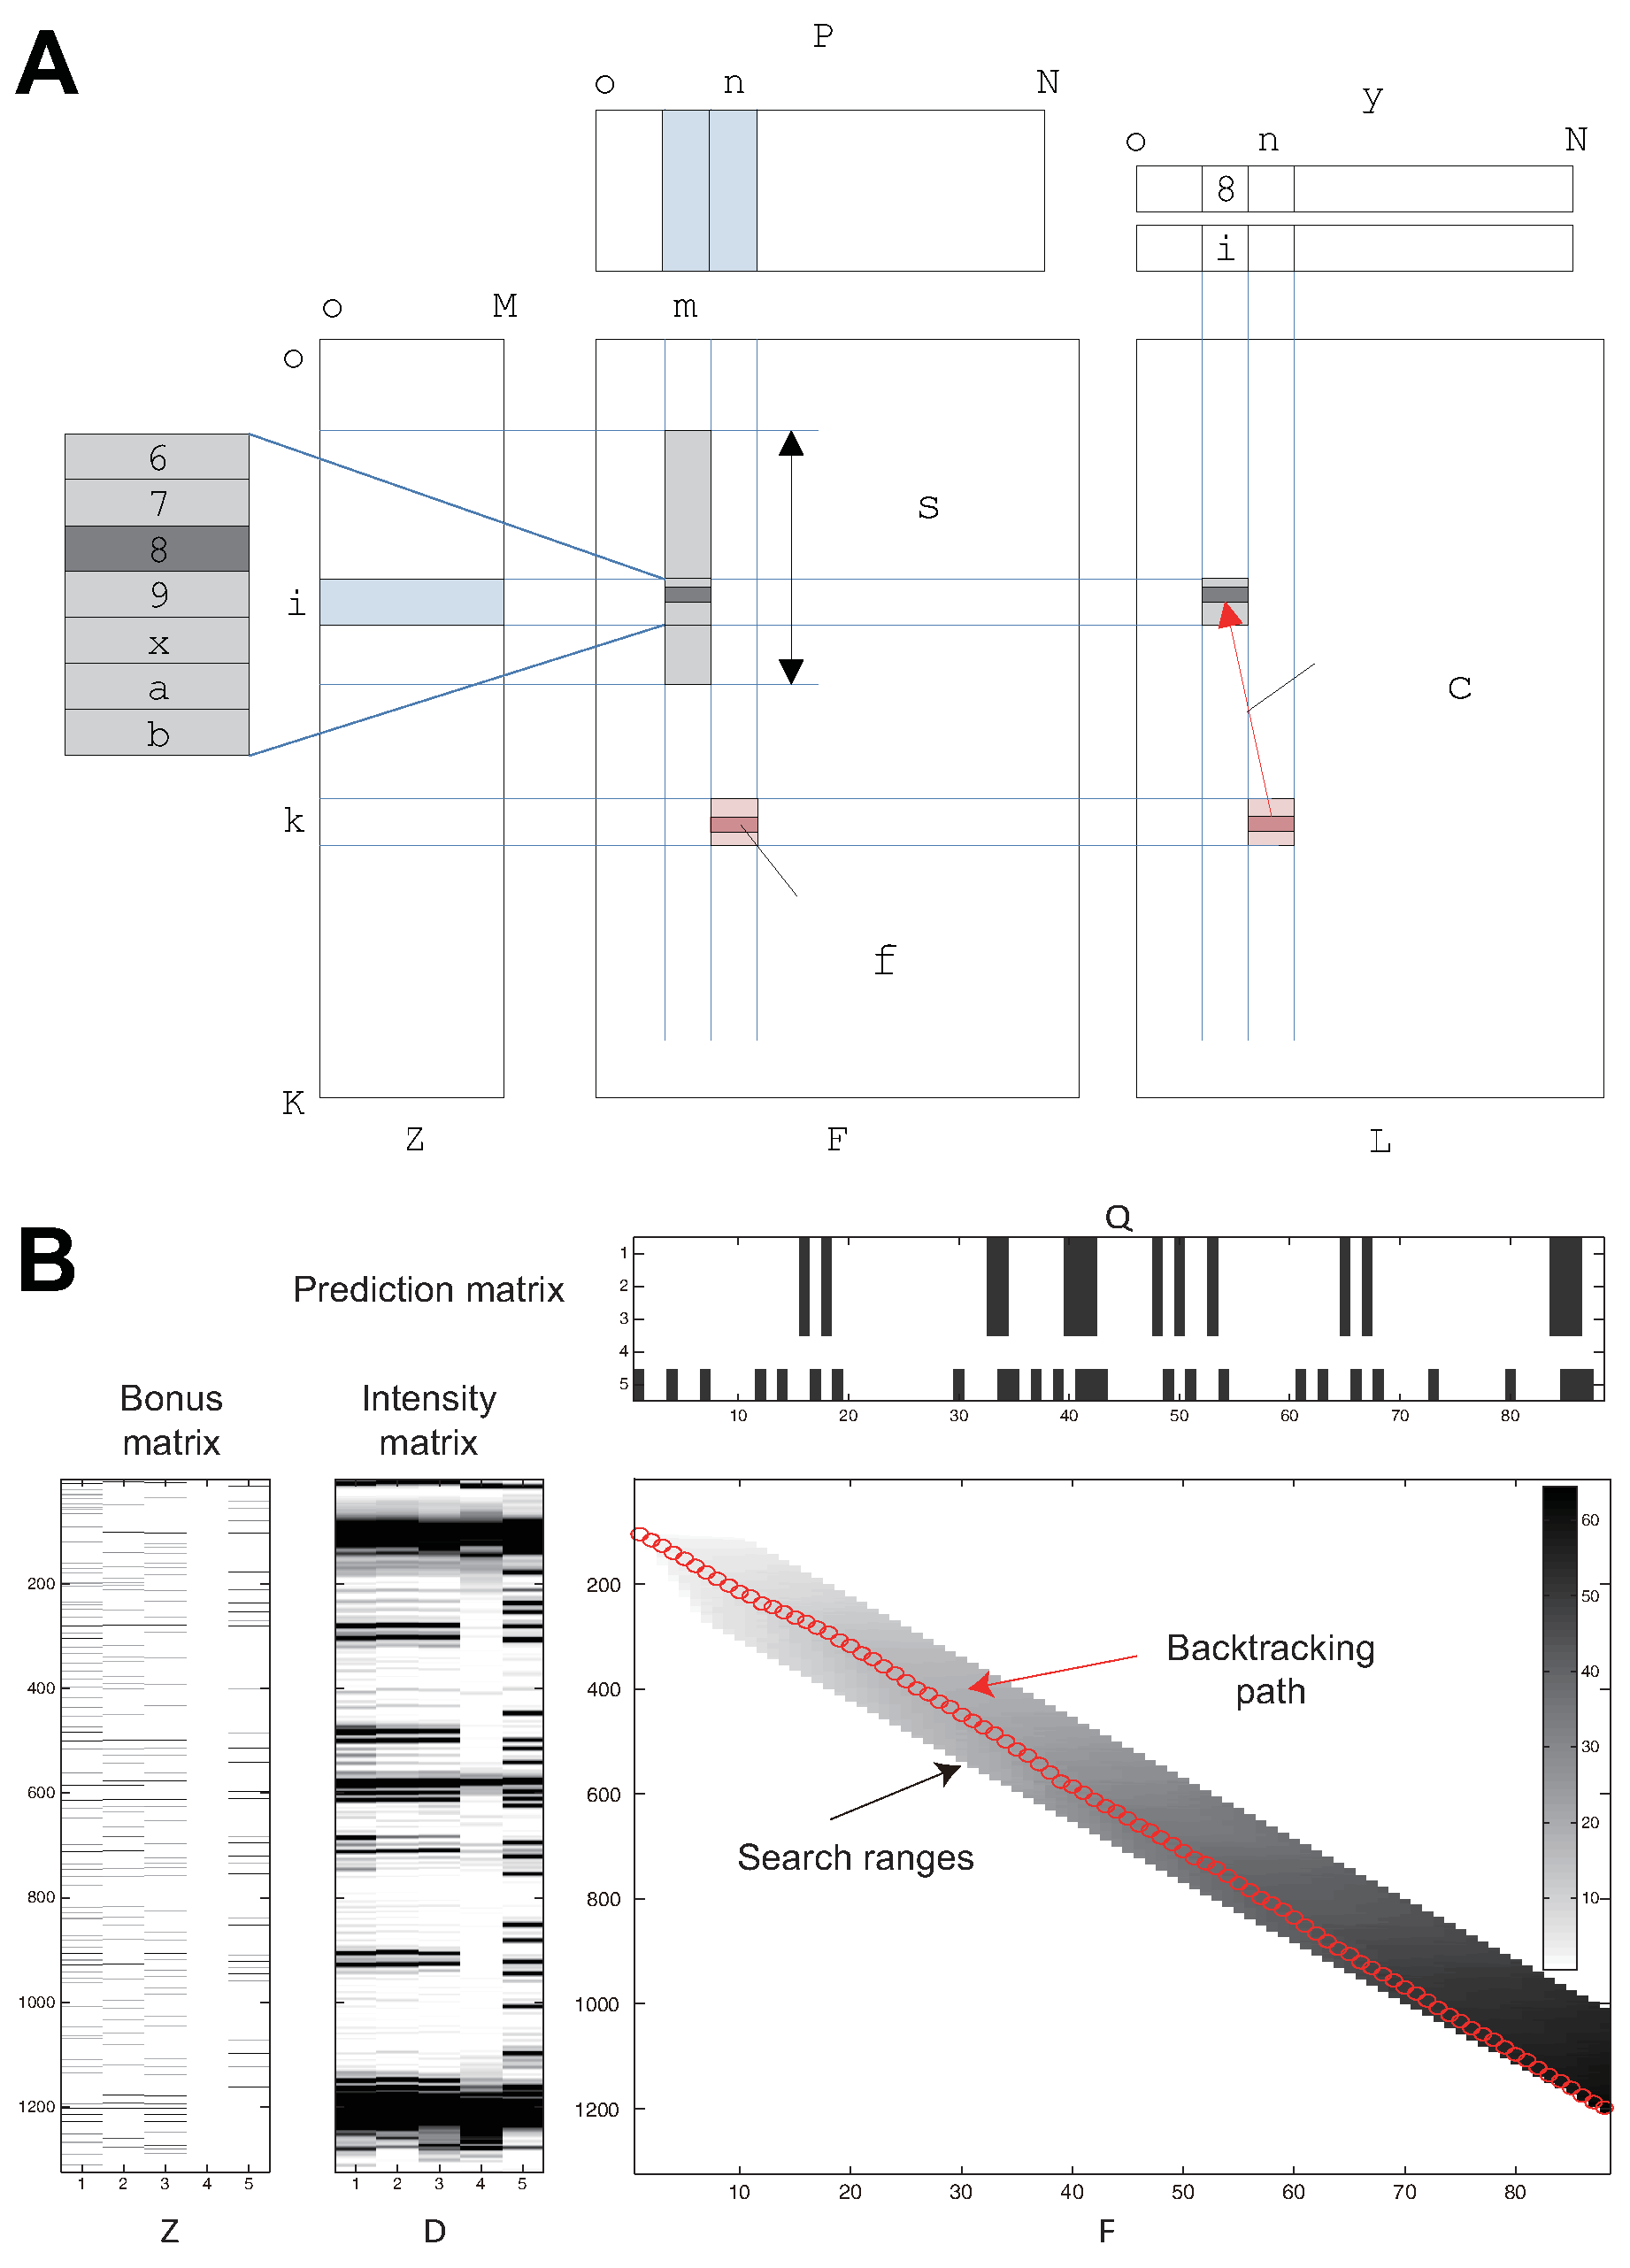
\includegraphics[width=0.85\linewidth]{figures/method_dp_formulation}
\caption{Formulation as dynamic programming. (\textbf{a}) $\bF(n,k,p)$ depends on $\bF(n-1,k',p')$ in the previous column and the gap bonus $S(n,k',k,n)$ between them. The best tuple $(k',p')$ that maximizes $\bF(n,k,p)$ is searched for in the range $k-2.5\rho \le k' < k; k'+p' < k+p$ and is stored in the backtracking matrices $\bL_k(n,k,p)$, $\bL_p(n,k,p)$. The computation of $S(n,k',k,p)$ is based on the bonus matrix $\bB$ and the prediction matrix $\bP$ (Section~\ref{ss:cost}). (\textbf{b}) Example. The data set used is `FMN Apatamer with single binding site.' $N=88$, $M=5$, $K=1324$. The backtracking path is represented by a series of red circles superimposed on the score matrix $\bF$; since $\bF$ is 3-dimensional, the figure alternatively represents a reduced matrix $\bF'$ defined by $\bF'(n,k)=\max_{p'} \bF(n,k,p')$. The output array $\by_k$, which stores the position of each circle, indicates the band locations.}
\label{f:dp-formulation}
\end{figure}
%%%%%%%%%%%%%%%%%%%%%%%%%%%%%%%%%%%%%%%%%%%%%%%%%%%%%%%%%%%%%%%%%%%%%%%%%%%%%%%%

\subsection{Formulation as dynamic programming}

\subsubsection{Basic motivation}
In essence, the band annotation problem is to select $N$ out of $K$ points and match them to peak locations (if at all possible) in an optimal way. This is similar to the problem of aligning two sequences $(1,2,\ldots,N)$ and $(1,2,\ldots,K)$ without allowing gaps for the latter.
\begin{align*}
\texttt{RNA sequence index    : -1--2---3...N...-}\\
\texttt{Measurement  index    : 123456789.......K}\\
\end{align*}
In the example above, the first three bands are located at 2, 5, and 9 time units. In order to find the most probable one among all such alignments, each possible alignment is given a score that represents its probabilistic likelihood. Dynamic programming can be utilized to find the solution set with the highest score, which in turn leads to the most likely locations of bands. More formally, define a matrix $\bF$ indexed by $n$ and $k$ ($1 \le n \le N$; $1 \le k \le K$) where the value $\bF(n,k)$ indicates the maximum score up to the band $n$ and position $k$. The matrix $\bF$ is filled up recursively:
%
\begin{equation}\label{e:F}
\bF(n,k) = \max_{\substack{k-2.5\rho \le k' < k}}\quad \left\{ \bF(n-1,k') + S(n,k',k) \right\}
\end{equation}
%
where $S(n,k',k)$ is the score attained by going from position $k'$ to $k$ for band $n$. The constraint on $k'$ in (\ref{e:F}) implies that a jump from $k'$ to $k$ is forward and its width is capped by a reasonable upper bound so that the entire search space can be narrowed down for efficient implementation. The search space is reduced even further into the profile of a moving window as shown in Figure~\ref{f:dp-formulation}, during our implementation.

\subsubsection{Primary profile}\label{sss:primary_profile}
In the previous section, our problem was formalized, but it fails to guarantee that the mapping from bands to candidate peaks is an one-to-one function. If there are two bands close to each other and only one peak is available for matching, both bands might be matched with the single peak at the same time. In order to prevent such circumstances, an additional search variable $p$ is introduced: the relative position of the matched peak to the band position $k$. The tuple $(n,k,p)$ corresponds to the instance in which the band $n$ is located at position $k$, and matched with the peak at $k+p$. The matrix $\bF$ is now redefined as a 3-dimensional matrix as follows:
%
\begin{equation}\label{e:F2}
\bF(n,k,p) = \max_{\substack{k-2.5\rho \le k' < k\\|p| < \rho/2\\k'+p' < k+p}}\quad \left\{ \bF(n-1,k',p') + S(n,k',k,p) \right\}
\end{equation}
%
The constraint $|p| < \rho/2$ is to restrict bands to be matched only with nearby peaks, and the last constraint $k'+p'<k+p$ means that two distinct bands cannot share the same peak. One problem that arises with the use of $p$ is that there should be $M$ such $p$'s for $M$ profiles, implying that the matrix $\bF$ should not be 3-dimensional but actually ($M+2$)-dimensional. However, this would make solving this problem too costly. As a compromise, the problem is simplified by choosing one primary profile among $M$ profiles so that $p$ is applied only to it; therefore $\bF$ may remain as a 3-dimensional matrix. Our software automatically determines the primary profile based on the data type with a preference for sequencing ladders. For our data sets, the last profile (a ddTTP ladder) was selected; without loss of generality, $\ba_M$ will be considered as the primary profile in the rest of this paper.

\subsubsection{Backtracking}
The backtracking matrices $\bL_k$, $\bL_p$ for finding the solution itself are given by
\begin{eqnarray}\label{e:L}
\bL(n,k,p)&=&(\bL_k(n,k,p), \bL_p(n,k,p)) \\
&=&\argmax_{\substack{k-2.5\rho \le k' < k\\|p| < \rho/2\\k'+p' < k+p}}\quad \left\{ \bF(n-1,k',p') + S(n,k',k,p) \right\} \nonumber
\end{eqnarray}
and respectively store the position $k$ and the relative peak location $p$ from which $\bF(n,k,p)$ is derived as in (\ref{e:F2}). The output array $\by$ is derived from $\bL_k$ and $\bL_p$ as follows:
%
\begin{eqnarray}\label{e:y}
\by(n) & = & (\by_k(n), \by_p(n)) \\
& = & \left\{
  \begin{array}{ll} \nonumber
    \argmax\limits_{k,p} \left\{\bF(N,k,p)\right\}, & \hbox{if $n = N$;} \\
    \bL(n+1, \by_k(n+1), \by_p(n+1)), & \hbox{$1 \le n \le N-1$.}
  \end{array}
\right.
\end{eqnarray}
%
The value of $\by_k(n)$ corresponds to the location of the $n$-th band in the input sequence $\bs$. Figure~\ref{f:dp-formulation} illustrates the proposed dynamic-programming formulation with an example.


\subsection{Description of score term}\label{ss:cost}
The score term in (\ref{e:F2}) consists of the following two components:
%
\begin{equation}\label{e:score-term}
S(n,k',k,p) = S_{\textrm{dist}}(n,k-k') + w_{\textrm{peak}} \cdot \bold{S}_{\textrm{peak}} (k,p) \cdot \bC(n, :)
\end{equation}
%
where $S_\textrm{dist}$ and $\bold{S}_\textrm{peak}$ are functions returning nonnegative values and $\bC(n,:)$ is the $n$-th row of the prediction matrix $\bC$. The dot product in the second term is a sum over all lanes $m$ from 1 to $M$. A coefficient $w_{\textrm{peak}}$ of 1.0 was discovered to give acceptable annotations in initial tests.


\subsubsection{Distance bonus term}

It is empirically supported that the length between consecutive locations, $k'$ and $k$, is quite evenly distributed. $S_{\textrm{dist}}$ is the bonus term that utilizes this fact and induces the dynamic programming to end up with regularly stretched output. In addition, observations on reference annotations suggest that a gap between two consecutive locations tends to be shorter when the preceding location corresponds to  `$\mathtt{G}$' in the RNA sequence. These observations lead to the definition of distance bonus term as follows:
%
\begin{equation}
S_{\textrm{dist}} (n,d) = {{f_{(\rho', {\rho \over 2})}(d)} \over {f_{(\rho', {\rho \over 2})}(0)}}
\end{equation}
%
where
%
\begin{equation}\nonumber
\rho' = \left\{
  \begin{array}{ll}
    {2 \over 3}\rho, &\hbox{if $\bs(n-1)=\mathtt{G}$;} \\
    \rho, &\hbox{otherwise}
  \end{array}
\right.
\end{equation}
%
and $f_{(\mu, \sigma)}$ is the density function of $N(\mu, \sigma)$. That is, $S_{\textrm{dist}}(n,d)$ reaches its maximum value 1 when $d = \rho'$ and decreases along a Gaussian curve as $d$ deviates from $\rho'$.


\subsubsection{Peak bonus term}
The second score term favors band locations near peaks of the electrophoretic profiles with a significant curvature. As the peak bonus is granted only for the profiles with a band at the location, $P(n,:)$ must be referred before actually adding up the bonuses as demonstrated in the equation (\ref{e:score-term}).
$\bold{S}_{\textrm{peak}}$ is a function that returns a nonnegative $M$-dimensional value where each of its entries represents the peak bonus from each profile:
%
\begin{equation}
\bold{S}_{\textrm{peak}}(k,p) = (S^1_{\textrm{peak}}(k), \ldots, S^{M-1}_{\textrm{peak}}(k), S^M_{\textrm{peak}}(k,p))
\end{equation}
%
where $S^m_{\textrm{peak}}$ stands for the bonus from matching a peak to a band in $\ba_m$, assuming such a band exists. The bonus is boosted for a greater curvature at the peak and the proximity of the peak to the band, so $S^m_{\textrm{peak}}$ is defined as the product of a Gaussian density function and an entry of $\bB$ corresponding to the peak:
%
\begin{equation}
S^m_{\textrm{peak}}(k) = \max_{\substack{|q| < \rho/2}} {{f_{(0, {\rho \over 5})}(q)} \over {f_{(0, {\rho \over 5})}(0)}} \cdot \bB(k+q, m)
\end{equation}
%
for $m < M$, and
%
\begin{equation}\label{e:peak-matching}
S^M_{\textrm{peak}}(k,p) = {{f_{(0, {\rho \over 5})}(p)} \over {f_{(0, {\rho \over 5})}(0)}} \cdot \bB(k+p, m) \cdot (M-1)
\end{equation}
%
As described above, this highly weighted peak bonus is taken from the primary profile (typically a sequencing ladder) rather than searching for optimal peak/band matches across all profiles to allow inclusion of peak information at reasonable computational expense. [A separate dynamic-programming-based band annotation algorithm was also tested which does not carry out the peak/band matching of eq. (\ref{e:peak-matching}) and gave slightly worse performance; see Supplemental Figure S1.]


\subsection{Reliability evaluation}\label{ss:reliability-evaluation}
While the presented band annotation method was found to be quite accurate, it was not perfect. We therefore sought a method to assess the reliability of automatically determined band locations prior to practical application. We devised a score to predict the quality of results. The idea behind the score is that when optimization of eq. (\ref{e:score-term}) fails to achieve the desirable solution, we typically see extraordinarily short or long distances between consecutive locations (little information from $S_\textrm{dist}$) or bands on the primary profile without proper matching to peaks (little information from $S_\textrm{peak}$). The $\escore$-score is defined with the following terms:
\begin{itemize}
\item $n_1$: number of bands on the primary profile without corresponding peak
\item $n_2$: number of gaps with length less than $\rho/4$, or greater than $2\rho$
\item $N^\textrm{peak}_M$: number of bands on the primary profile predicted by $\bC$
\item $\escore = 1 - {\max({{n_1} \over N^\textrm{peak}_M}, {{n_2} \over {K-1}})}$
\end{itemize}
$\escore$-score is a value between 0 and 1 and conservatively estimates the number of normalities in the output relative to the number of bands and locations. Greater $\escore$-score means less abnormalities in the output which is believed to result from output digressing from the correct answer, so it can be expected that output with $\escore$ closer to 1 would be more reliable than output with smaller $\escore$. The relationship between $\escore$-score and accuracy is presented in the Results section.

\begin{comment}
\subsection{Implementation}
We implemented the proposed method in the MATLAB programming environment (The MathWorks, http://www.mathworks.com) and are making it freely available for download at http://hitrace.stanford.edu.
(To be filled with data preparation...)
\end{comment}

%%%%%%%%%%%%%%%%%%%%%%%%%%%%%%%%%%%%%%%%%%%%%%%%%%%%%%%%%%%%%%%%%%%%%%%%%%%%%%%
% TABLE 1
%%%%%%%%%%%%%%%%%%%%%%%%%%%%%%%%%%%%%%%%%%%%%%%%%%%%%%%%%%%%%%%%%%%%%%%%%%%%%%%
\begin{table}
\processtable{High-throughput RNA structure mapping data sets analyzed by the proposed method (total 522 profiles and 47210 bands). Excluding the last line, there are 95 data sets. More details of these 95 data sets are described in \citet{lee2014eterna}. %The last data set is from a study on a 187-nt ribozyme.
\label{t:data}}
{\begin{tabular}{lcccc}
\toprule
Name& \# profiles & \# nt & \# bands per profile & \# total bands \\
\midrule
R45$^a$  &60&	108&	88&	5280\\
R46$^a$  &80&	108&	88&	7040\\
R47$^b$  &90&	112&	92&	8280\\
R47B$^b$  &36&	112&	92&	3312\\
R48$^b$  &96&	112&	92&	8832\\
R49$^b$  &18&	112&	92&	1656\\
R49B$^c$  &48&	115&	95&	4560\\
R50$^c$  &54&	115&	95&	5130\\
R43$^d$  &40&	98&	78&	3120\\
%HDV$^e$ & 4& 187 & 187 & 748\\
\botrule
\end{tabular}}
{$^a$Flavin mononucleotide (FMN) aptamer with single binding site~\citep{lee2014eterna}; $^b$FMN aptamer with single binding site II; $^c$FMN binding branches; $^d$The backwards C%; $^e$NMIA (SHAPE) modification of the hepatitis delta virus (HDV) ribozyme
%Abbreviations: FMN, flavin mononucleotide
}
%Abbreviations: SRP, signal recognition particle conserved domain; P4-P6, P4-P6 domain of the Tetrahymena group I ribozyme; DMS, dimethyl sulfate; CMCT, 1-cyclohexyl-3-(2-morpholinoethyl) carbodiimide metho-p-toluenesulfonate; SHAPE, selective hydroxyl acylation analyzed by primer extension.}
\end{table}




\end{methods}

\section{Results}\label{s:result}
%%%%%%%%%%%%%%%%%%%%%%%%%%%%%%%%%%%%%%%%%%%%%%%%%%%%%%%%%%%%%%%%%%%%%%%%%%%%%%%
% BAND ASSIGN
%%%%%%%%%%%%%%%%%%%%%%%%%%%%%%%%%%%%%%%%%%%%%%%%%%%%%%%%%%%%%%%%%%%%%%%%%%%%%%%
\begin{figure}
\centering
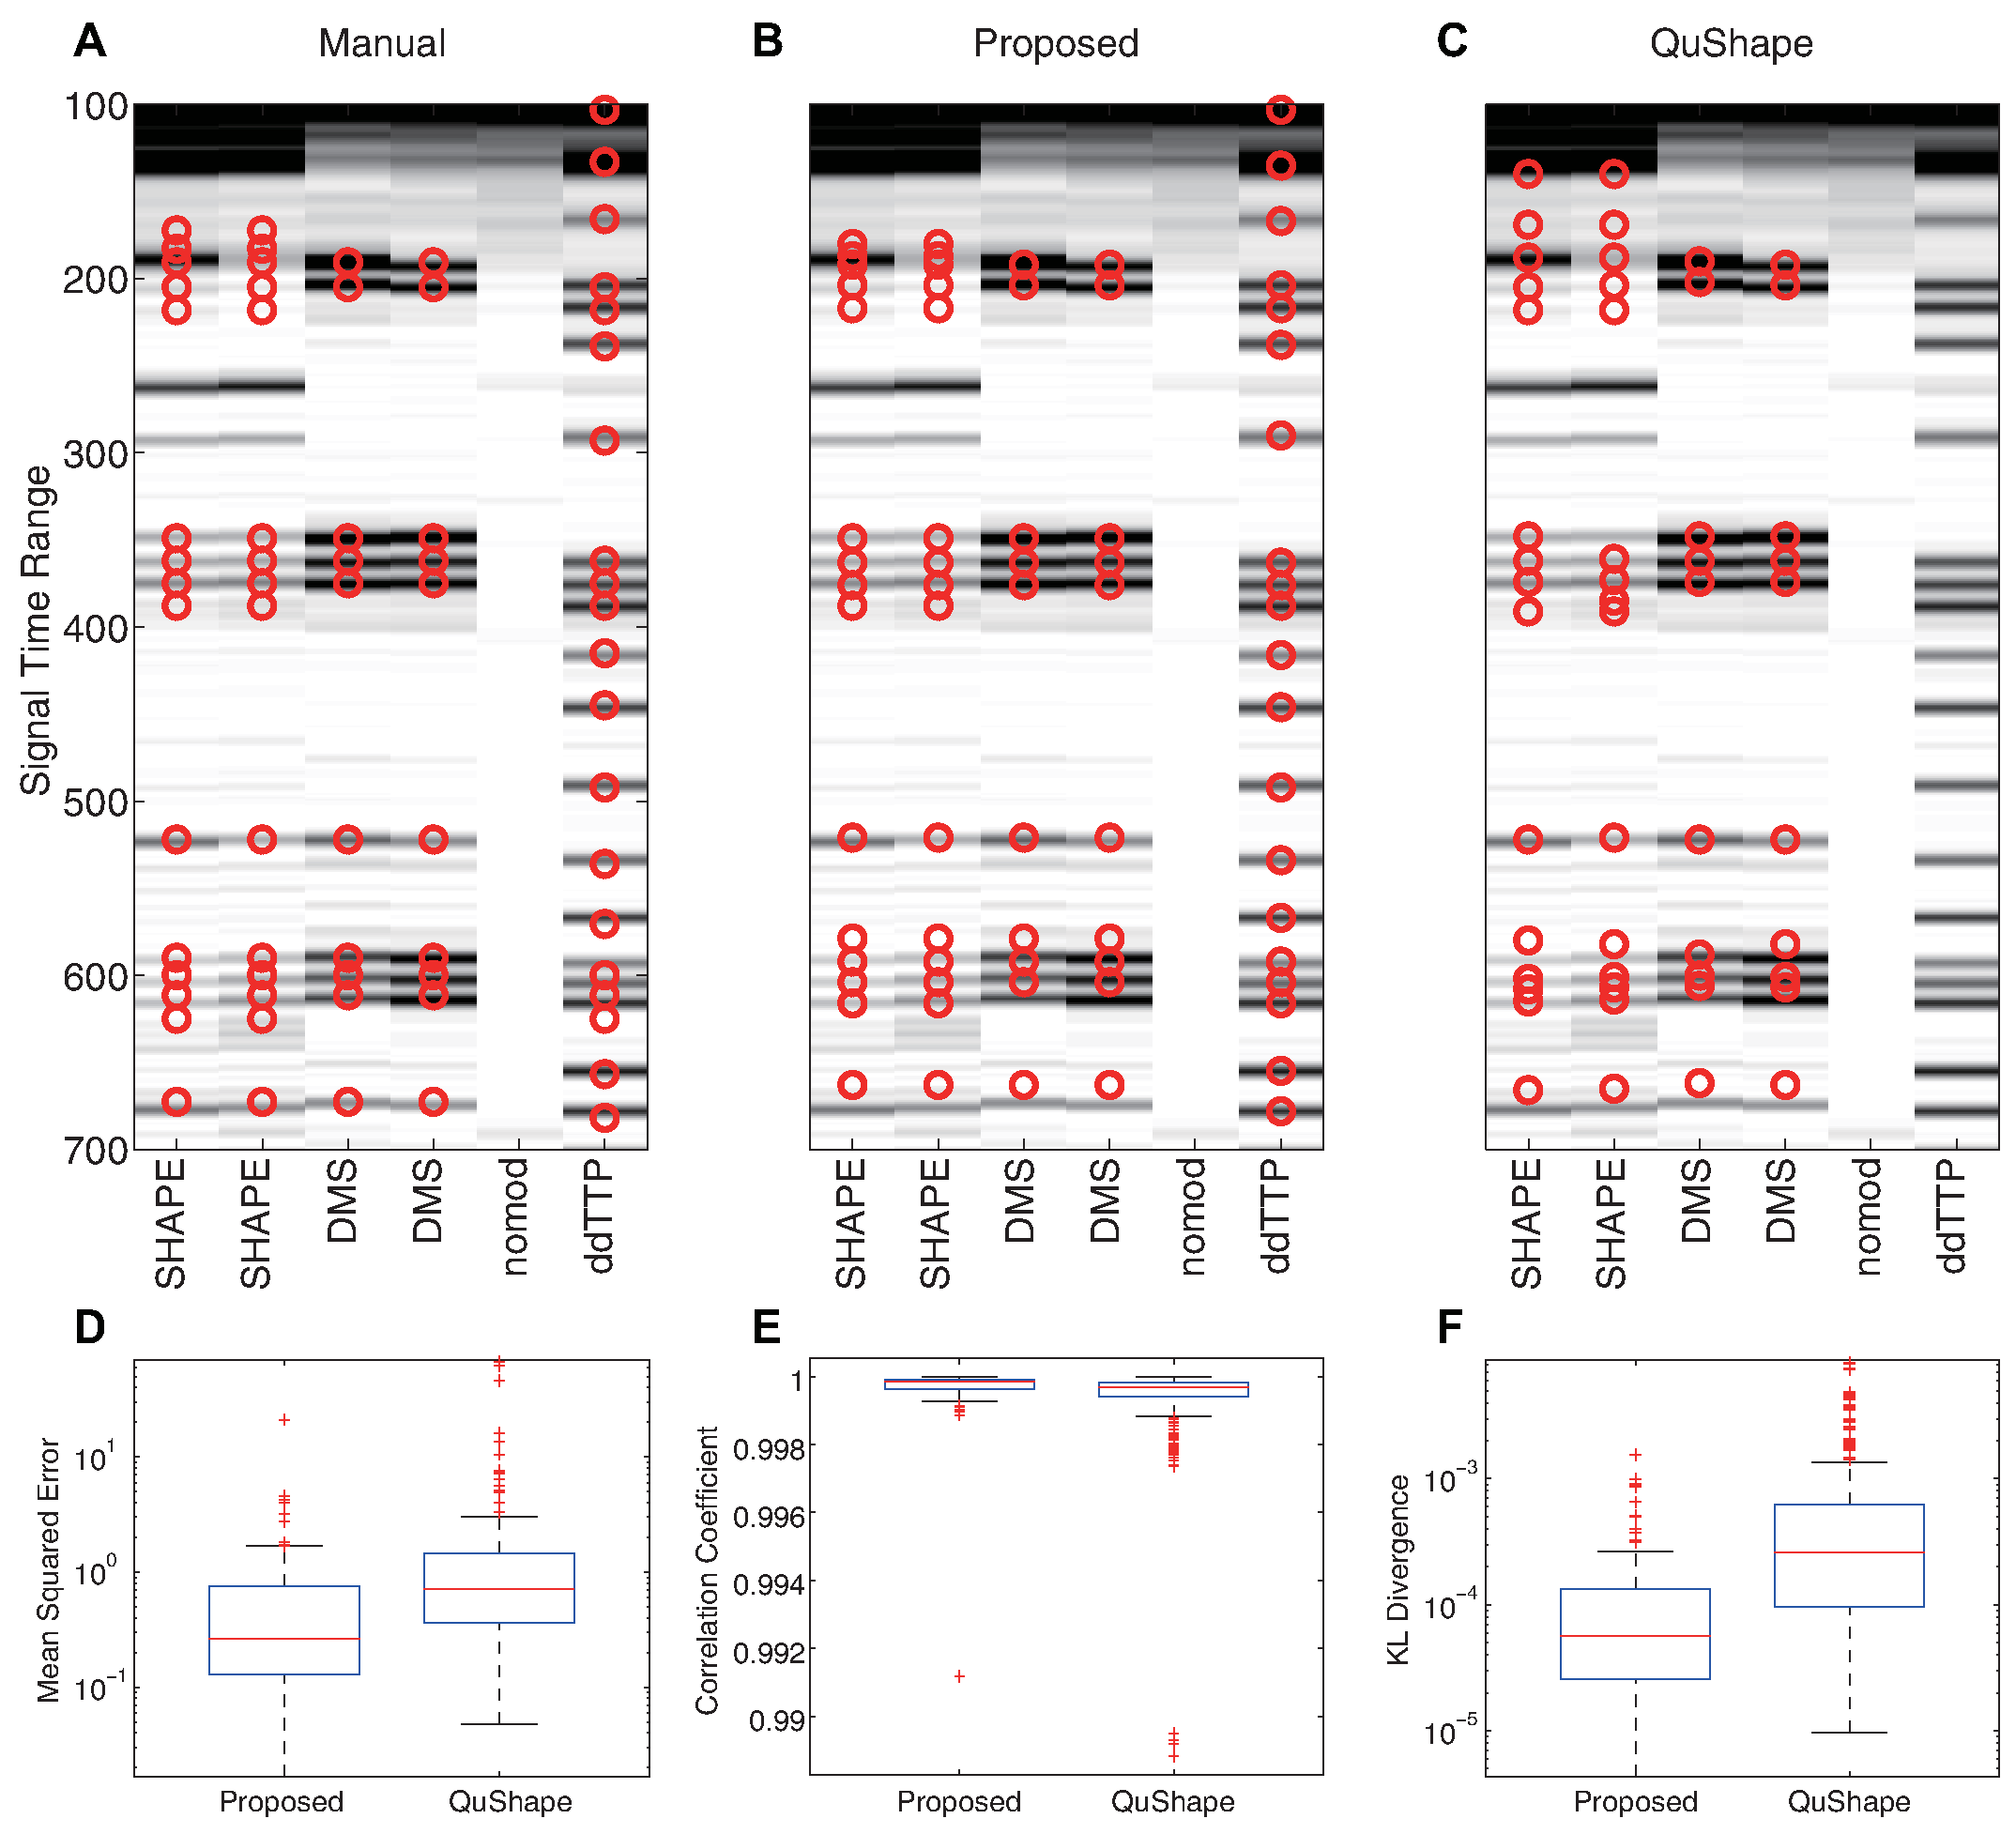
\includegraphics[width=0.9\linewidth]{figures/result_band_assign4}
\caption{Determination of band locations. (A) Reference (manual) annotation. Red circles represent band locations. (B) The band locations determined by the proposed method. (C) The band locations found by QuShape~\citep{Karabiber2013}. (D) Mean squared error (MSE) (E) Pearson's correlation coefficient (F) KL divergence}
\label{f:band-assign}
\end{figure}
%%%%%%%%%%%%%%%%%%%%%%%%%%%%%%%%%%%%%%%%%%%%%%%%%%%%%%%%%%%%%%%%%%%%%%%%%%%%%%%

%%%%%%%%%%%%%%%%%%%%%%%%%%%%%%%%%%%%%%%%%%%%%%%%%%%%%%%%%%%%%%%%%%%%%%%%%%%%%%%
% PEAK AREA
%%%%%%%%%%%%%%%%%%%%%%%%%%%%%%%%%%%%%%%%%%%%%%%%%%%%%%%%%%%%%%%%%%%%%%%%%%%%%%%
\begin{figure}
\centering
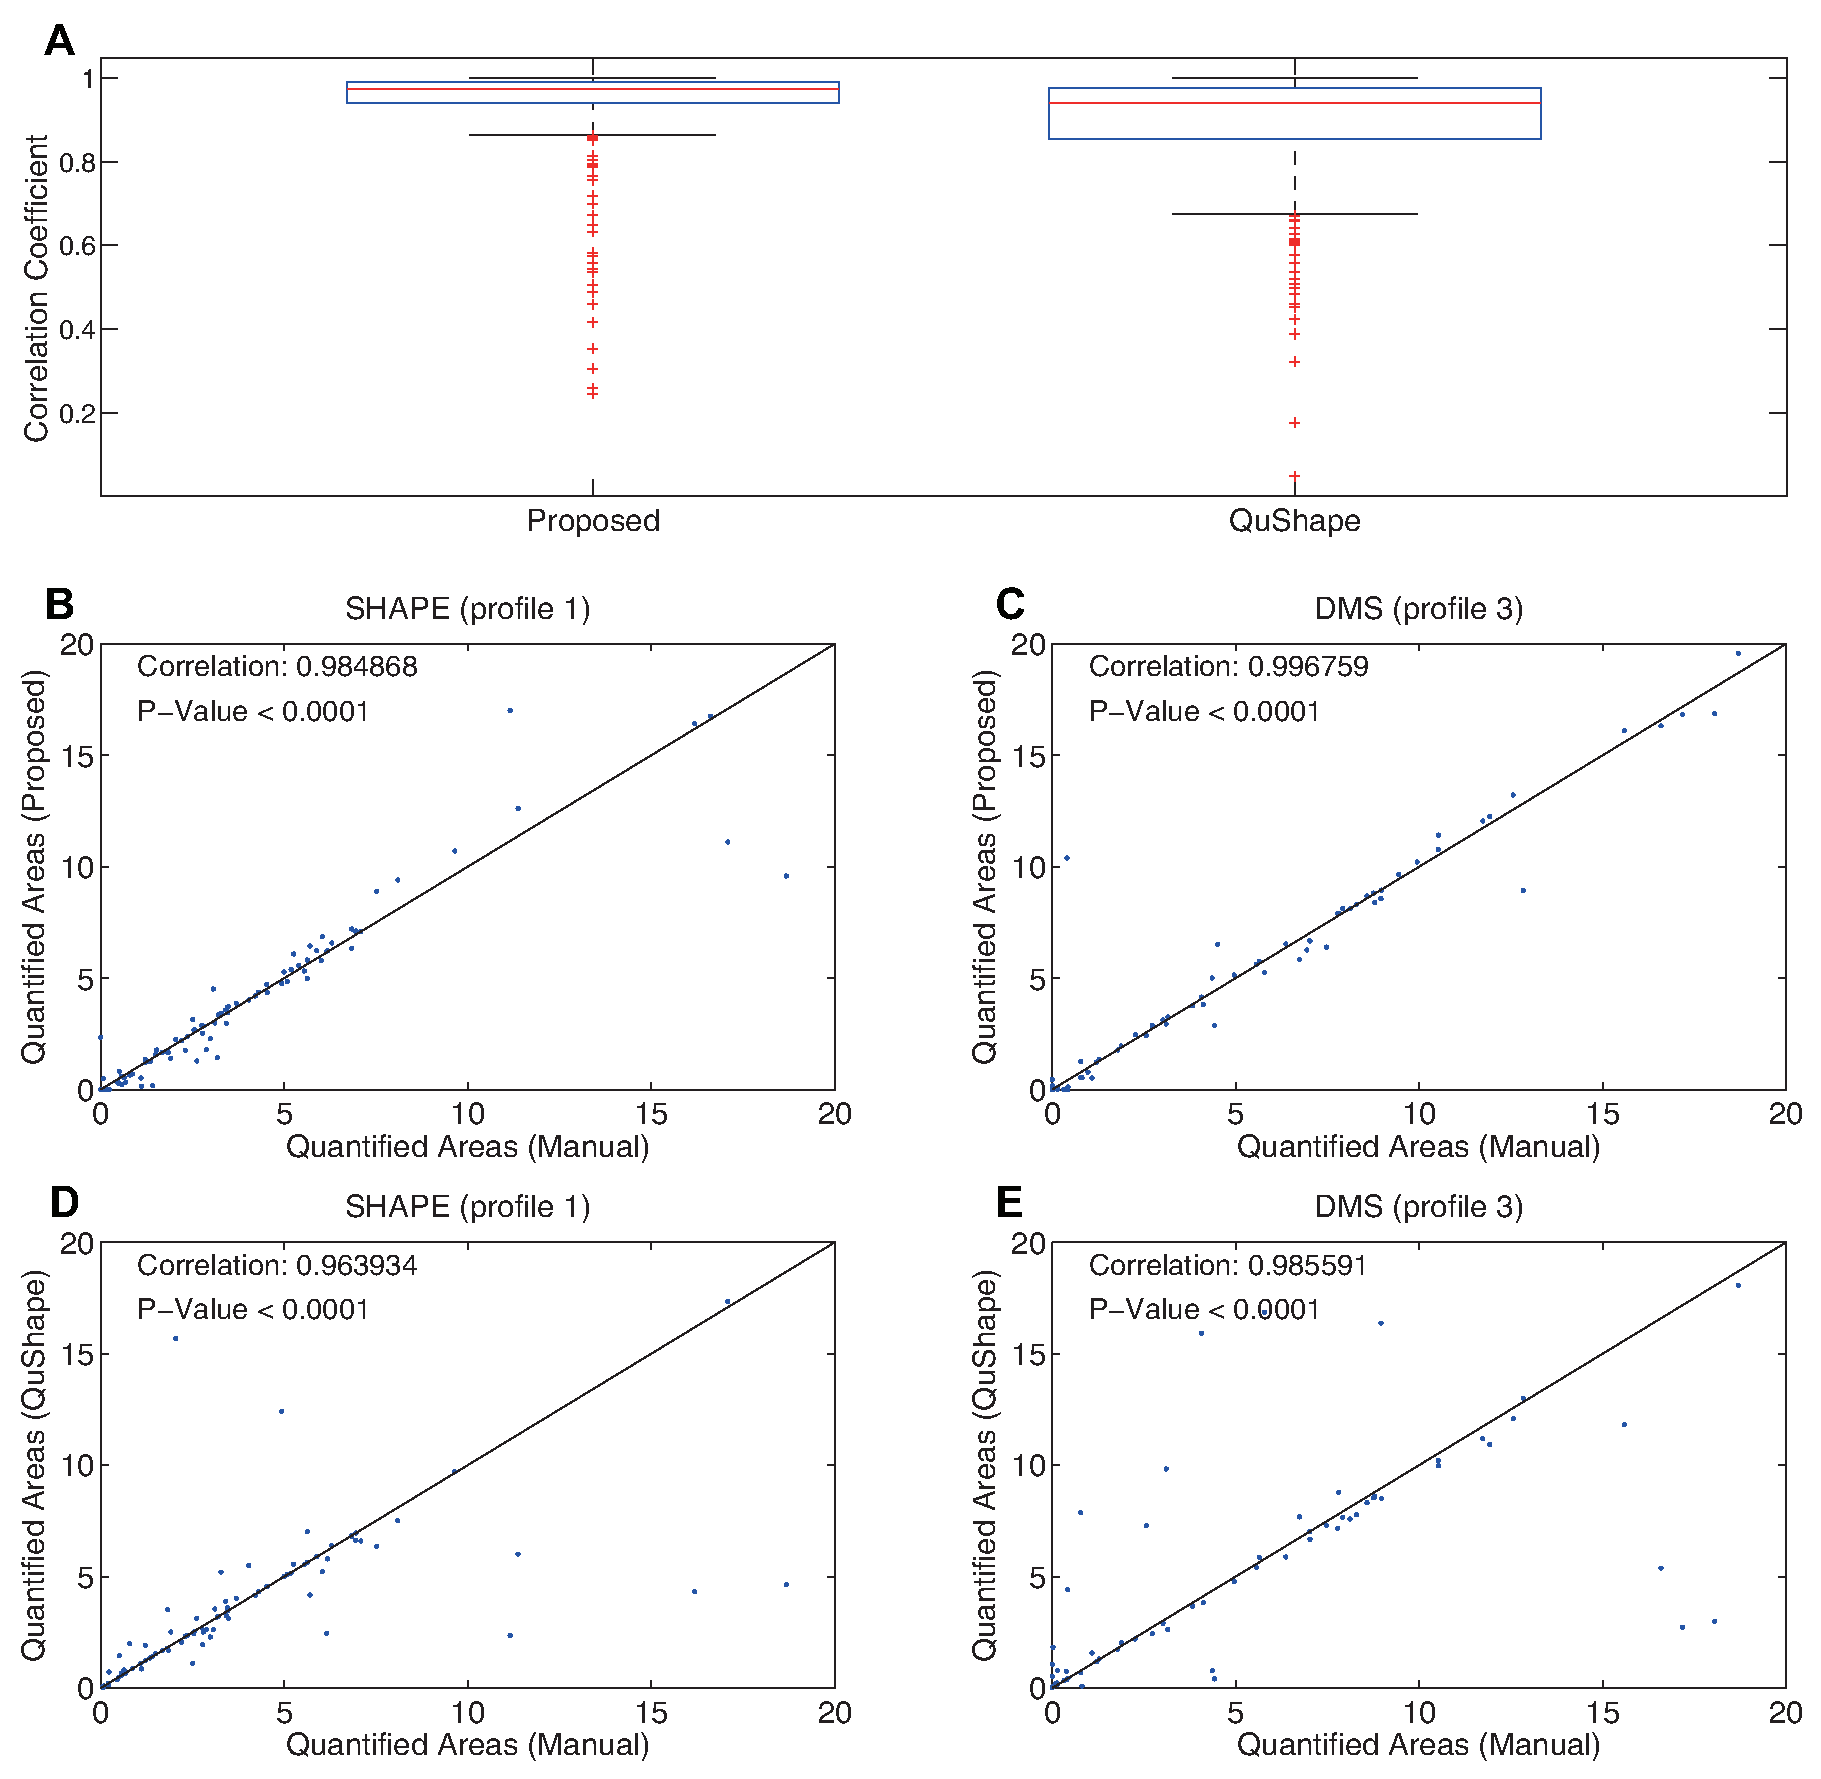
\includegraphics[width=0.9\linewidth]{figures/result_peak_area4}
\caption{Accuracy of quantifying peak areas. (\textbf{a}) The left box plot represents the distribution of the Pearson's correlation coefficients between the manually quantified areas and those quantified by the proposed method over the 95 data sets. The right box plot shows the distribution of the correlation coefficients between the areas quantified manually and by QuShape. (\textbf{b}--\textbf{c}) Correlation of the reference and the quantified areas by the proposed method for data set `FMN Binding Branches' is shown for profiles 1 (SHAPE) and 3 (DMS). (\textbf{d}--\textbf{e}) Correlation of the reference and the areas quantified by QuShape for the same data set.
}
\label{f:peak-area}
\end{figure}
%%%%%%%%%%%%%%%%%%%%%%%%%%%%%%%%%%%%%%%%%%%%%%%%%%%%%%%%%%%%%%%%%%%%%%%%%%%%%%%

\newcommand{\bP}{{\mathbf{P}}}


\subsection{Robust determination of band positions}\label{ss:band-position}
Figure~\ref{f:band-assign}(a)--(c) shows the electrophoretic profiles annotated with band locations by three different methods: reference, proposed, and QuShape~\citep{Karabiber2013}, respectively. The reference annotation was based an expert assignments carried out at the time of data acquisition~\citep{lee2014eterna} QuShape was chosen as the comparison target for its superior accuracy in band annotation relative to other software we tested, FAST and ShapeFinder (data not shown); nomod and ddTTP profiles were used as references (RXS1, BGS1) while running QuShape. Visual inspection suggests that the proposed method produces annotations more compatible with the reference. In this profile, the annotation determined by QuShape deviates from the reference position, particularly near the beginning of sequence.

To generally and quantitatively assess the accuracy of automated band annotation, we applied the proposed method and QuShape to 95 data sets acquired in the EteRNA project (Table \ref{t:data}). For both methods, we computed the mean squared error (MSE) of the band locations determined by the proposed method with respect to the reference locations, in units of average distance between locations. For a sense of scale, the typical MSE achieved by expert annotation is 0.15, based on comparisons of different experts' annotations with each other and to next-generation-sequencing-based measurements, where sequence annotation is unambiguous \citep{Kladwang2014}; see Supplemental Fig. S1. In our experience, a band annotation result with MSE lower than 0.5 typically requires no or a small number single-click corrections. The box plots in Figure~\ref{f:band-assign}(d)--(f) and individual MSE values (Supplemental Tables S1 and S2) reveal that the proposed method outperforms QuShape across the data sets. For example, the median MSE of the proposed method is 0.37, under the target value of 0.5, compared to 1.8 from QuSHAPE. As separate metrics of accuracy, we measured the Pearson's correlation coefficient and the Kullback-Leibler (KL) divergence between the reference and computationally determined band positions.  Again, the average correlation coefficient of the proposed method is 1.92 times closer to 1, and the average KL divergence is 5.49 times smaller. These results quantitatively confirm what we observed qualitatively on using these tools: significantly less manual intervention is needed with the proposed method compared to QuShape.


\subsection{Accurate peak-area quantification}\label{ss:peak-area}
In the RNA structure mapping pipeline, the band annotation is followed by peak deconvolution, which fits each band with a Gaussian curve and outputs the quantified area of the band. To see how these final band quantification results are impacted by the band annotation method, we calculated Pearson's correlation coefficients between band areas quantified based on the band annotation found by the proposed method and those quantified based on the reference annotation. We also repeated the calculation with the band intensities quantified by QuShape. For fair comparison, we applied the same peak deconvolution software (HiTRACE; \citealp{Yoon2011}) to these three methods.

As one example, Figure~\ref{f:peak-area}(b) and (c) shows the correlation of results between the proposed method and reference for a specific data set (FMN Binding Branches) for two chemical modification strategies (SHAPE and DMS).and Figure~\ref{f:peak-area}(d) and (e) shows the correlation between the QuShape and reference results, which is visually worse than the proposed method in both cases. Over all the data sets, Figure~\ref{f:peak-area}(a) and Supplemental Table S1 gives the distribution of the Pearson's correlation coefficients. The median correlation coefficient for the proposed method is 0.969, which is higher than that for QuShape (0.896) and the distribution for the proposed method shows smaller variance. This observation suggests that using the proposed band annotation can significantly enhance the accuracy of band quantification. 


\begin{comment}
%%%%%%%%%%%%%%%%%%%%%%%%%%%%%%%%%%%%%%%%%%%%%%%%%%%%%%%%%%%%%%%%%%%%%%%%%%%%%%%
% HDV RESULT
%%%%%%%%%%%%%%%%%%%%%%%%%%%%%%%%%%%%%%%%%%%%%%%%%%%%%%%%%%%%%%%%%%%%%%%%%%%%%%%
\begin{figure}
\centering
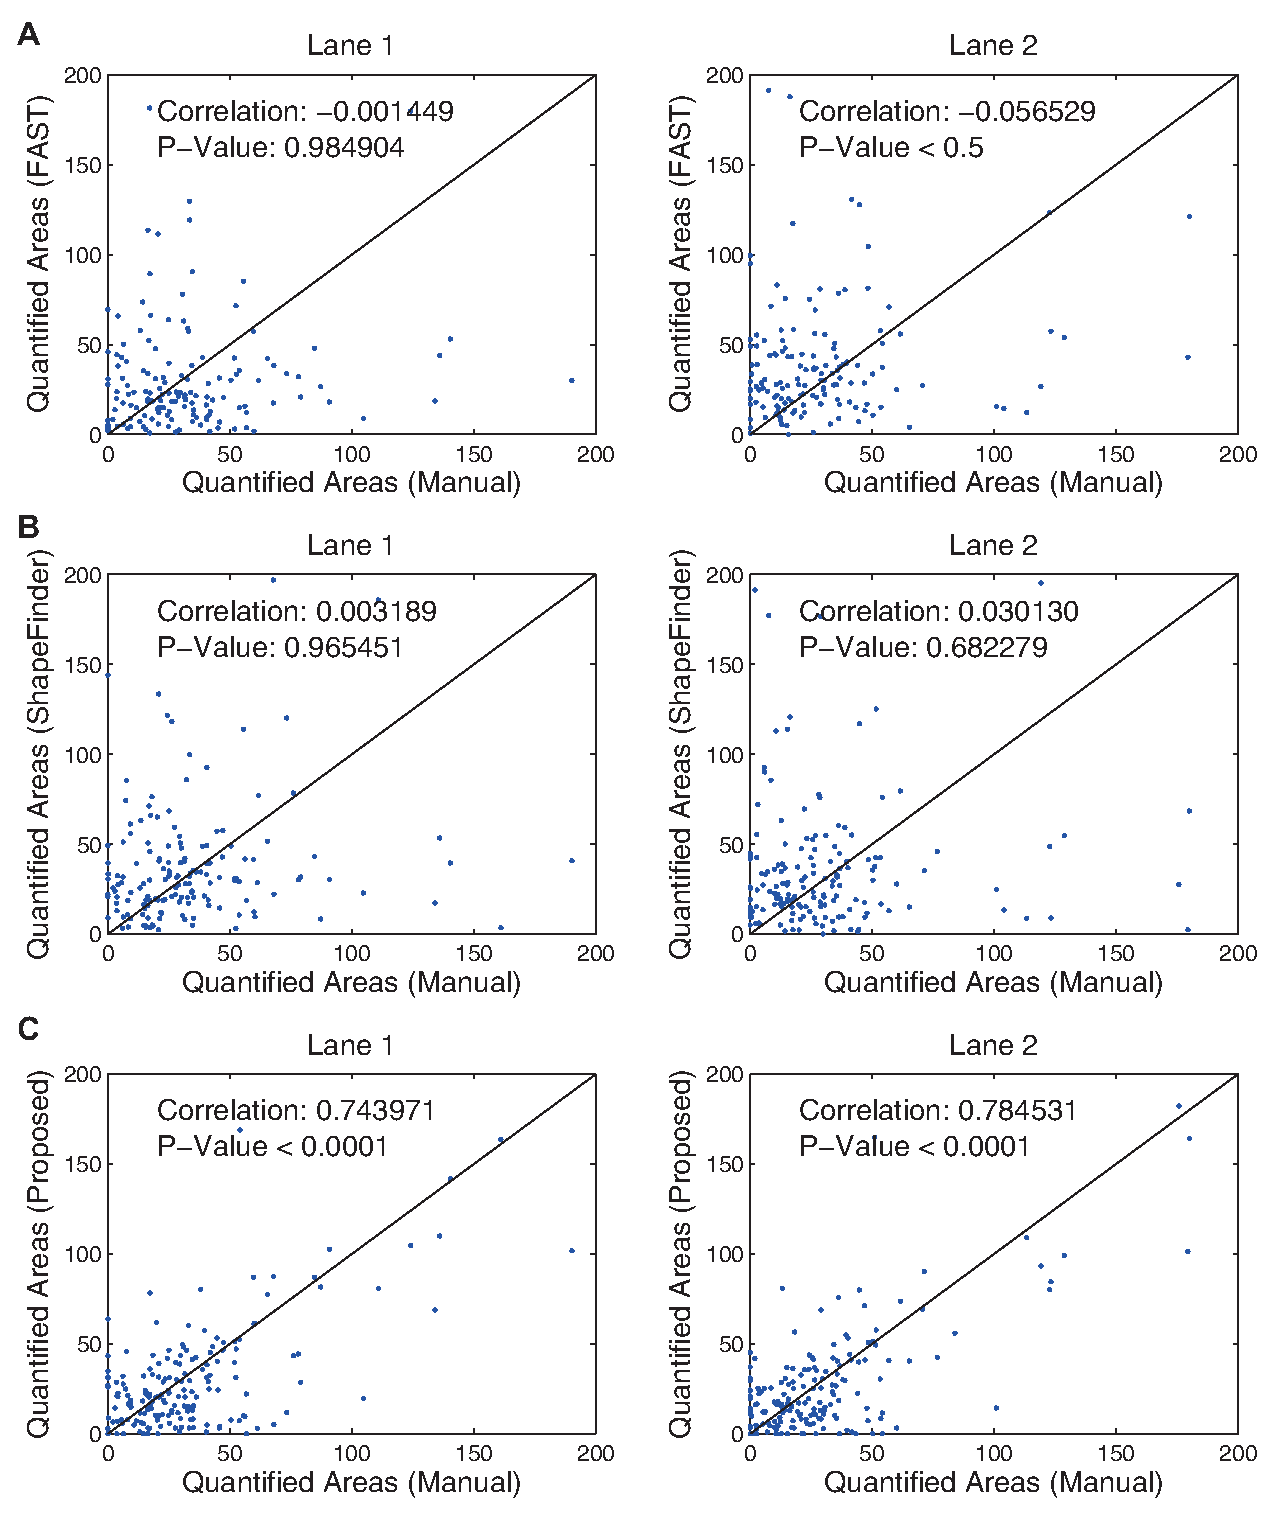
\includegraphics[width=\linewidth]{figures/result_hdv_result3}
\caption{Assessing band annotation results from 187-nt HDV data set. (\textbf{a}--\textbf{c}) Correlation between the areas quantified manually and by FAST, ShapeFinder, and the proposed method over two profiles, respectively.}
\label{f:hdv-result}
\end{figure}
%%%%%%%%%%%%%%%%%%%%%%%%%%%%%%%%%%%%%%%%%%%%%%%%%%%%%%%%%%%%%%%%%%%%%%%%%%%%%%%

\subsection{Results in longer RNAs}
To test the proposed method with a longer RNA molecule, we used a chemical mapping data set from a study on the NMIA (SHAPE) modification of the hepatitis delta virus (HDV) ribozyme (187-bp). For this data set, we included the FAST software~\citep{Pang2011} in comparison. FAST has a hard-wired requirement for ddGTP as reference ladder and could not be used for the other 95 data sets presented earlier (they contained ddTTP profiles instead).

We repeated the experiments presented in Sections~\ref{ss:band-position} and \ref{ss:peak-area} for this HDV data set. The proposed method substantially outperformed FAST and ShapeFinder in terms of MSE (proposed: 1.14, ShapeFinder: 321.03, and FAST: 142.12), although its MSE is higher than those for shorter sequences (Figure~\ref{f:band-assign}(d)). 


\emph{I DON'T THINK WE SHOULD SHOW THESE R VALUES -- EVEN FOR OUR NEW METHOD, THEY ARE NOT ACCEPTABLE}
Figure~\ref{f:hdv-result}(a)-(c) shows the correlation of the reference areas with band areas quantified by the proposed method, ShapeFinder, and FAST, respectively. The band areas quantified by the proposed method show a high degree of correlation with the reference ($r= 0.744$ and $0.785$), whereas the two other methods give unsatisfactory results ($r< 0.05$). 

Figure~\ref{f:hdv-result-detail} shows the distribution of errors in predicted band locations over the position of residues in the HDV data set. This is to check if there is any systematic bias in band annotation on the residue position. The middle diagram represents the mapping between the reference band locations and those determined by the proposed method. The upper and lower plots show the position errors for the proposed method and FAST, respectively. For the proposed method, the errors near the start location tends to be larger than those in the middle. According to our experience, there exist very high-intensity bands in the starting and ending portion of a profile, which hinders even the manual band annotation. The larger error near these segments in a profile may be due to these high-intensity bands. The error pattern in the result from FAST shows a different pattern, and the largest errors appear near residues 40--50. Overall, the errors from the proposed method were consistently lower than those from FAST.


%%%%%%%%%%%%%%%%%%%%%%%%%%%%%%%%%%%%%%%%%%%%%%%%%%%%%%%%%%%%%%%%%%%%%%%%%%%%%%%
% HDV RESULT DETAIL
%%%%%%%%%%%%%%%%%%%%%%%%%%%%%%%%%%%%%%%%%%%%%%%%%%%%%%%%%%%%%%%%%%%%%%%%%%%%%%%
\begin{figure}
\centering
	\psfrag{r}[][][0.5]{$\rho$}
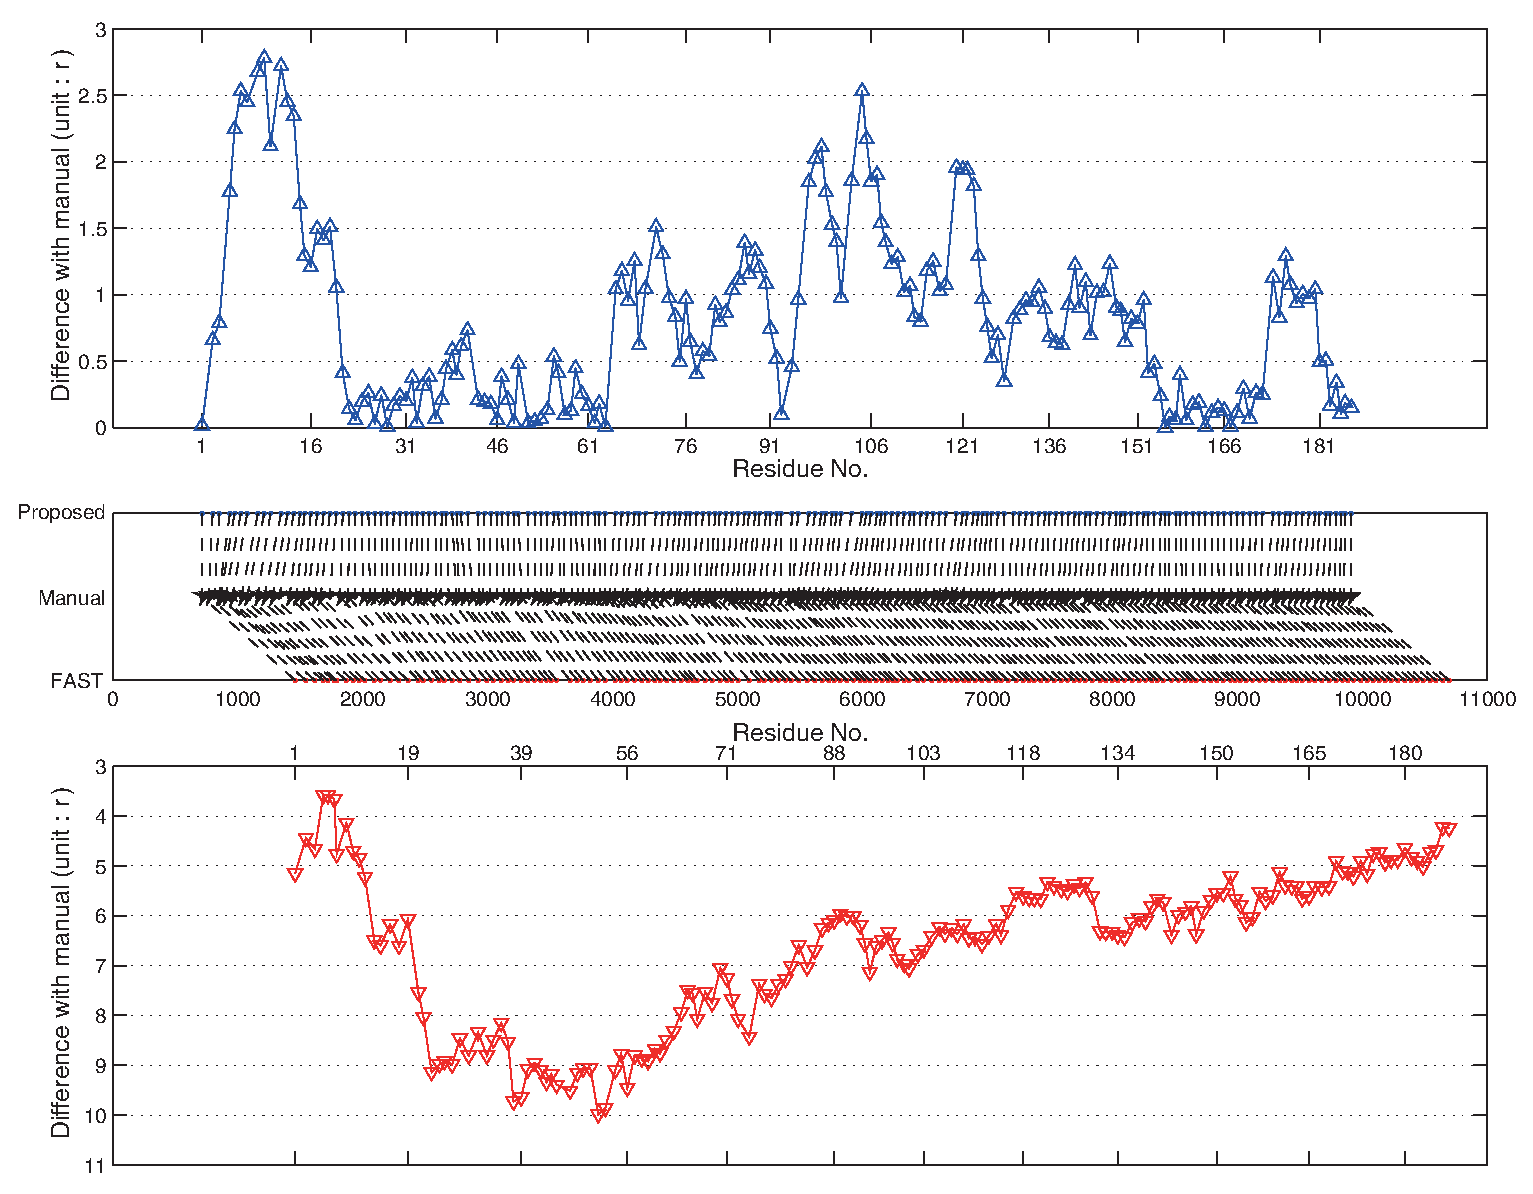
\includegraphics[width=\linewidth]{figures/result_hdv_result_detail2}
\caption{Error in band positions with respect to the reference band locations for 187-nt HDV data. Upper plot: error over residue positions for the proposed method; middle: mapping between the reference and computationally predicted band locations; lower: error over residue positions for FAST.}
\label{f:hdv-result-detail}
\end{figure}
%%%%%%%%%%%%%%%%%%%%%%%%%%%%%%%%%%%%%%%%%%%%%%%%%%%%%%%%%%%%%%%%%%%%%%%%%%%%%%%
\end{comment}


%%%%%%%%%%%%%%%%%%%%%%%%%%%%%%%%%%%%%%%%%%%%%%%%%%%%%%%%%%%%%%%%%%%%%%%%%%%%%%%
% E-SCORE MSE
%%%%%%%%%%%%%%%%%%%%%%%%%%%%%%%%%%%%%%%%%%%%%%%%%%%%%%%%%%%%%%%%%%%%%%%%%%%%%%%
\begin{figure}
\centering
	\psfrag{x}[][][0.7]{$\escore$-score}
	\psfrag{y}[][][0.7]{$\escore=1$}
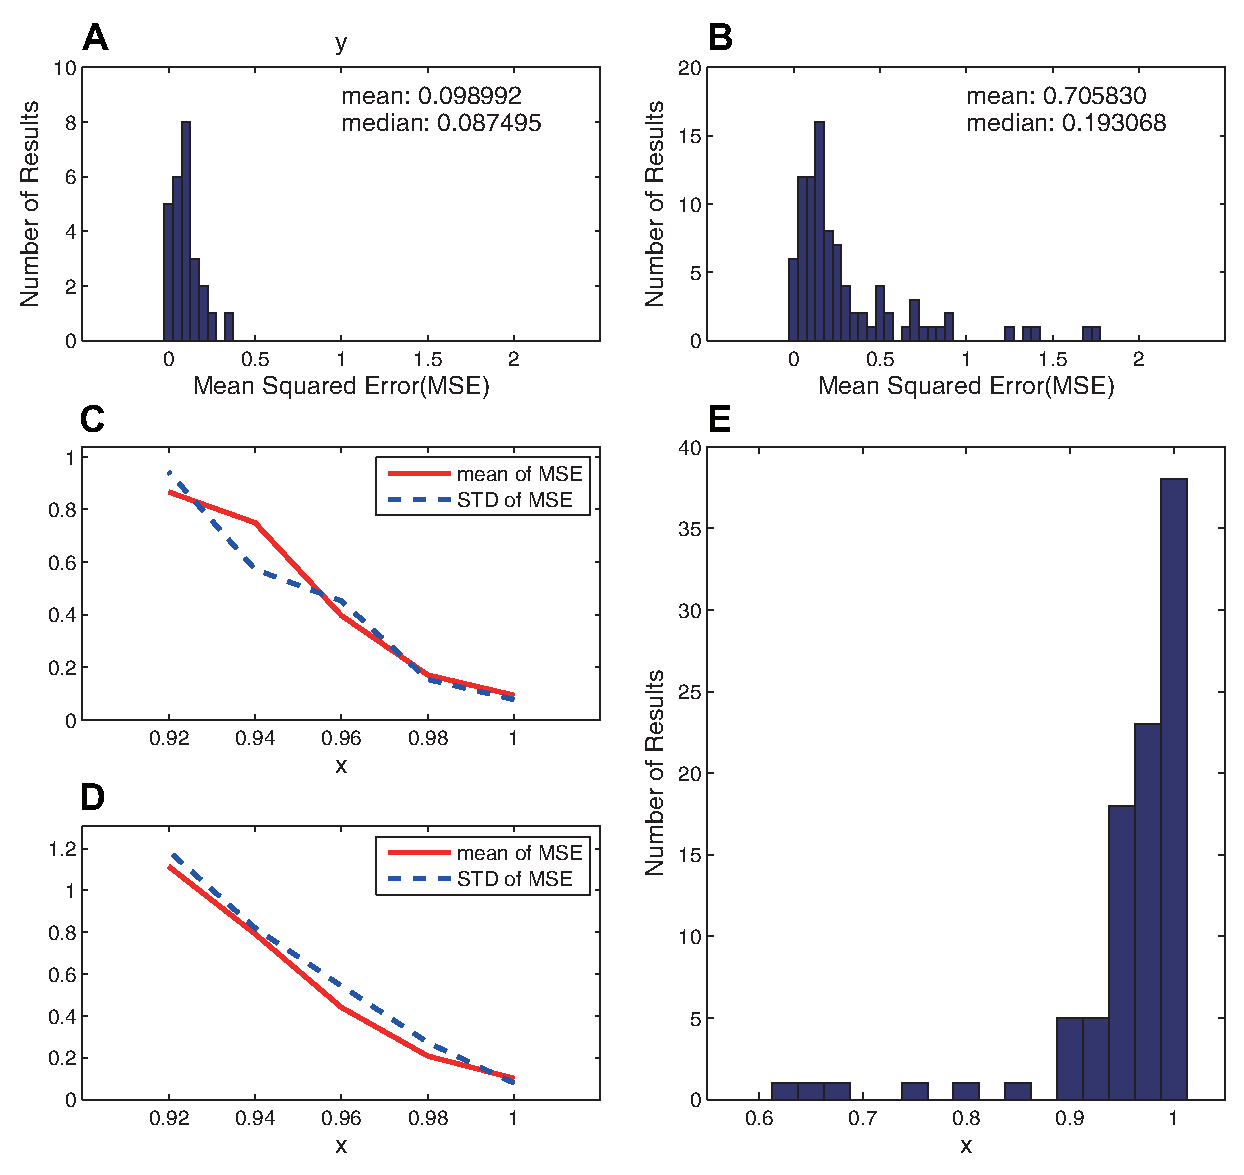
\includegraphics[width=0.9\linewidth]{figures/result_escore_mse4}
\caption{(\textbf{a}) Distribution of MSE for the results with 1 $\escore$-score. (\textbf{b}) Distribution of MSE for the whole 95 results. (5 results with MSE $> 2$ are ommited for better demonstration) (\textbf{c}) Trends of mean and standard deviation of MSE with respect to $\escore$-score over artificial data generated from a single original data set. (\textbf{d}) Trends of mean and standard deviation of MSE with respect to $\escore$-score for artificial data generated from the whole 95 data sets. (\textbf{e}) Distribution of $\escore$-score over 95 data sets.}
\label{f:escore-mse}
\end{figure}
%%%%%%%%%%%%%%%%%%%%%%%%%%%%%%%%%%%%%%%%%%%%%%%%%%%%%%%%%%%%%%%%%%%%%%%%%%%%%%%

\subsection{$\escore$-score reliability metric predicts MSE accuracy}

In Section~\ref{ss:reliability-evaluation}, we proposed $\escore$-score to evaluate the quality of results from our method. We assessed the use of $\escore$-score based on its ability to predict the accuracy of the band annotations compared to gold standard annotations, quantitatively evaluated as mean squared error (MSE). Figure~\ref{f:escore-mse}(a) show the distribution of the MSEs where (a) only contains results satisfying $\escore = 1.0$; the MSE values are substantially smaller than those in (b), which includes all 95 data sets.  For example, all 26 results under constraint $\escore=1.0$ have MSE below 0.5 as shown in (a), confirming that a `perfect' $\escore$-score essentially guarantees high quality of band annotations; furthermore, 50 out of 51 results with $\escore>0.97$ have MSE below 0.5 (even the one exception has MSE less than 1). In addition to this experimental test, artificial data sets were generated based on the original data sets through random convolution in terms of amplitude and interval for further verification. Figure~\ref{f:escore-mse}(c)--(d) show the trends of mean and standard deviation of MSE with respect to $\escore$-score, where (c) comes from artificial data generated from a single data set whereas artificial data involved in (d) is generated from the whole 95 data sets. The trends shown in (c) and (d) further confirm that a lower $\escore$-score corresponds to MSE values with higher (worse) mean and standard deviation. Figure~\ref{f:escore-mse}(e) shows the histogram of the $\escore$-scores over the 95 data sets prepared. Overall, 39\%  of the data sets have $\escore$-score equal to 1, and 84\%  have $\escore$-score greater than 0.97, suggesting that poor $\escore$-scores and subsequent detail manual correction will be encountered in a minority of cases.

\begin{comment}
%%%%%%%%%%%%%%%%%%%%%%%%%%%%%%%%%%%%%%%%%%%%%%%%%%%%%%%%%%%%%%%%%%%%%%%%%%%%%%%
% TABLE 2
%%%%%%%%%%%%%%%%%%%%%%%%%%%%%%%%%%%%%%%%%%%%%%%%%%%%%%%%%%%%%%%%%%%%%%%%%%%%%%%
\begin{table}
\processtable{Additional data sets and results from tests.
\label{t:additional_results}}
{\begin{tabular}{lcccc}
\toprule
Name & \# profiles & \# bands per profile & MSE & $\escore$-score \\
\midrule
GIR1 noref 	& 21 & 199 & 0.09 & 0.99 \\
GIR1 ref 		& 21 & 225 & 0.12 & 0.98 \\
AdoCbl noref 	& 16 & 179 & 0.61 & 0.97 \\
AdoCbl ref 	& 16 & 205 & 0.68 & 0.90 \\
VS noref 		& 48 & 195 & 0.16 & 0.96 \\
VS ref 		& 48 & 233 & 0.12 & 0.96 \\
SAM noref 	& 32 & 103 & 0.09 & 0.96 \\
SAM ref 		& 32 & 143 & 0.09 & 0.96 \\
HTP noref 	& 32 & 79  & 0.05 & 1.00 \\
HTP ref 		& 32 & 116 & 0.05 & 1.00 \\
Tbox 		& 20 & 141 & 0.34 & 0.98 \\
tRNA 		& 20 & 119 & 0.63 & 0.83 \\
cdiAMP 		& 36 & 171 & 0.16 & 0.99 \\
16S 			& 8  & 125 & 0.21 & 0.98 \\
C19 			& 16 & 319 & 0.18 & 0.99 \\
tC19 		& 16 & 248 & 0.01 & 1.00 \\
tC19Z 		& 16 & 248 & 0.01 & 0.99 \\
C1Lig 		& 7  & 167 & 0.04 & 1.00 \\
Hox5 		& 9  & 261 & 0.11 & 0.99 \\
Hox9D 		& 16 & 296 & 0.44 & 0.99 \\
L-21			& 20 & 413 & 2.00$^a$ & 0.98 \\
\botrule
\end{tabular}}
{$^a$An extraordinary result mainly caused by a misalignment between profiles (to be discussed in the discussion section) 
}
\end{table}
%%%%%%%%%%%%%%%%%%%%%%%%%%%%%%%%%%%%%%%%%%%%%%%%%%%%%%%%%%%%%%%%%%%%%%%%%%%%%%%
\end{comment}

\subsection{Results in longer, biological RNA sequences}
In an effort to test the proposed method's compatibility with a wide array of high-throughput RNA structure mapping data sets, we prepared sample experimental datasets of biologically derived RNAs. These additional 21 data sets include Class I ligase ~\citep{Bagby01122009}, L-21 ScaI ribozyme ~\citep{Shi2009}, a four-way junction from E. coli 16S rRNA ~\citep{tian2014nature}, RNA replicases (C19, tC19 and tC19Z) ~\citep{Wochner08042011}, human Hox transcripts $5^\prime$ UTR (Hox5 and Hox9D189) (Nature, in press) and RNA Puzzle entries (\#5-10, and 12) ~\citep{Cruz01042012}. In each dataset, complete sets of chemical modifier reactions (nomod, SHAPE, DMS, CMCT) and reference ladders (ddNTPs) are present. In addition, an HDV ribozyme segment studied previously \citep{Pang2011} allowed direct comparison to the FAST software (Supplemental Fig. S2). These RNAs had lengths up to 400 nucleotides, significantly longer than the ~100-nt EteRNA designs (Table \ref{t:data}). Despite this increase length, the band annotation results from the proposed method were still highly consistent with the reference expert annotation. Excluding an abnormal result from L-21 caused by an experimental issue that disallowed alignment of sequencing ladders, the maximum of MSE is only 0.68. Furthermore, two worst MSE values (0.68 and 0.63) and two lowest $\escore$-scores (0.83 and 0.90) coincide in the results for AdoCbl(noref) and tRNA, confirming $\escore$-score's utility. 

\begin{comment}
%%%%%%%%%%%%%%%%%%%%%%%%%%%%%%%%%%%%%%%%%%%%%%%%%%%%%%%%%%%%%%%%%%%%%%%%%%%%%%%
% REACTIVITY COMPARISON
%%%%%%%%%%%%%%%%%%%%%%%%%%%%%%%%%%%%%%%%%%%%%%%%%%%%%%%%%%%%%%%%%%%%%%%%%%%%%%%
\begin{figure}
\centering
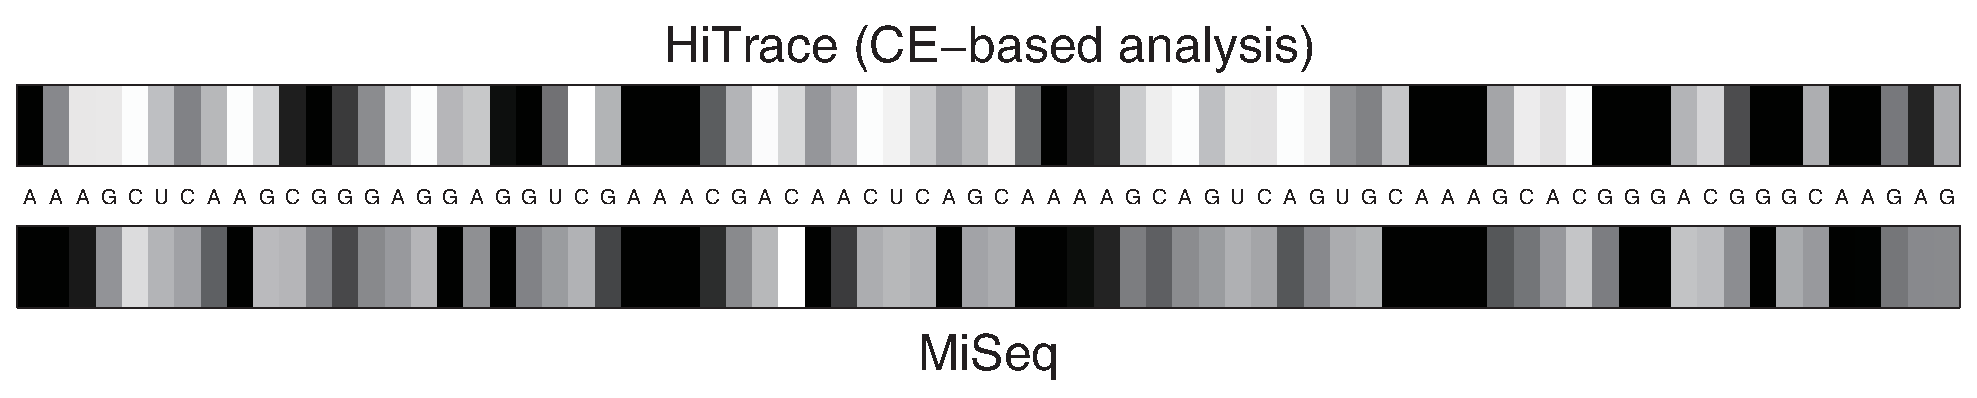
\includegraphics[width=\linewidth]{figures/reactivities}
\caption{Heatmaps those represent the reactivity values obtained by CE-based analysis and MiSeq, respectively. The data set used is 'C-BACK' sequence.}
\label{f:reactivity-comparison}
\end{figure}
%%%%%%%%%%%%%%%%%%%%%%%%%%%%%%%%%%%%%%%%%%%%%%%%%%%%%%%%%%%%%%%%%%%%%%%%%%%%%%%

\subsection{Reactivity comparison with miseq}
For the final step of verification, we compared the reactivity data obtained by using the proposed method in conjunction with HiTrace, with that obtained by using MiSeq method. In spite of their separated experimental samples and environments, the two reactivity data sets share a same trend as shown in Figure~\ref{f:reactivity-comparison}, evidencing the consistency between the two distinct analyses in terms of their final results.

\end{comment}


\section{Discussion}\label{s:discussion}
%\emph{ WE SHOULD HAVE A SECTION EXPLAINING THE POWER OF USING MULTIPLE TRACES TO DERIVE A CONSENSUS BAND ANNOTATION-- RHIJU}

%\subsection{Use of RNA secondary structure information for band annotation}
%\emph{ I WOULD DE-EMPHASIZE THIS -- PERHAPS NOT EVN MAKE IT A SEPARATE SECTION. WHAT IF YO UHAVE AN RNA WITH UNKNWON SECONDARY STRUCTURE? OR WITH MULTIPLE SECONDARY STRUCTURES?}
%In the band annotation procedure for an RNA sequence, the proposed method constructs the band prediction matrix $\mathbf{P}$ based on the RNA's secondary structure predicted by the Vienna RNA package~\citep{hofacker2003vienna}. Although the secondary structure prediction software typically matches most experimental profiles closely, there may exist cases (\eg, complicated pseudoknots) in which the prediction quality is low or even fails. In such cases, using secondary structure information may lead to incorrect band annotation, but through preliminary filtering we can reduce the possibility of inaccurate annotation.

The proposed method for band annotation is unique in its ability to take into account all available CE profiles; prior methods (such as those available in QuShape and FAST) have focused on a single profile at a time with a reference profile if needed. The distinctive robustness of the proposed method is primarily attributed to this capability to integrate information across profiles. The method does require an accurate alignment of all profiles prior to band annotation. Our prior work \citep{Yoon2011} described a different dynamic programming algorithm to accomplish this annotation based on standards co-loaded with each sample. In well over 100 data sets analyzed here, we saw only one case where inter-profile alignment was problematic (L-21 ScaI group I intron) and required manual intervention. Therefore, our alignment and annotation results herein confirm that automated analysis of RNA structure mapping CE measurements can now be routinely achieved.

To flag cases with uncertain automated band annotation, we have introduced the $\escore$-score for reliability estimation. According to our experiences, given any data set for CE analysis, the band annotations with $\escore > 0.97$ are almost always reliable and can be safely adopted for final steps of band quantitation whereas the results with $\escore \le 0.97$ are less likely to reliable. Informally, we have encountered data sets in which even expert annotation is ambiguous and has required special additional experiments (such as co-loading sequencing ladders in the same color as the sample) to resolve \citep{tian2014nature}. This suggests that automated band annotation cannot improve much further; a valuable development would be reliability estimates for specific subsets of bands rather than a global number.

The proposed algorithm has order of $NK$ time and space complexity, and the practical time demand of band annotation was resonable in our experiments. The proposed method was implemented in the MATLAB programming environment (The MathWorks, http://www.mathworks.com), and under the experimental setup used (sequential execution on a Intel core i5 4570 processor with 8-GB main memory), the total time demand of annotating bands in all the 95 data sets did not exceed 4 min (for each data set, mean 2.2837 sec; median 2.2707 sec).



\section{Conclusion}\label{s:conclusion}
In the analysis of CE profiles, band annotation has remained the most time-consuming step, due to the lack of robust computational tools for automating the process. Using a dynamic-programming approach, the proposed algorithm can find an optimal arrangement of bands in a given CE profile, under a scoring scheme suitable for high-throughput CE experiments with multiple profiles. On over 100 CE data sets including designed and biological RNAs, the proposed method identified the band positions matching the reference positions with acccuracy sufficiently high as to obviate or significantly reduce manual correction. Finally, the quality of the band positions are well predicted by $\escore$-score, flagging unreliable annotations to the user.



\section*{Acknowledgments}
The authors thank Menashe Elazar at the Glenn Laboratory at Stanford University for providing the HDV ribozyme data.

\paragraph{Funding\textcolon}
This work was supported in part by the National Research Foundation of Korea funded by the Ministry of Education, Science and Technology (Grant No. 2011-0009963 and No. 2011-0000158 to SY) and in part by a Burroughs-Wellcome Foundation Career Award at the Scientific Interface (to RD for computational work).


\bibliographystyle{natbib}
%\bibliographystyle{reference}
%\bibliographystyle{unsrt}
\bibliography{reference}


\end{document}


